\documentclass[11pt]{article}
\usepackage[margin=1in]{geometry}
\usepackage[T1]{fontenc}
\usepackage{lmodern}
\DeclareUnicodeCharacter{03BC}{\ensuremath{\mu}}
\usepackage{amsmath,amssymb,amsthm,mathtools}
\usepackage{booktabs,array,multirow,tabularx}
\usepackage{graphicx}
\usepackage[font=small,labelfont=bf]{caption}
\usepackage{subcaption}
\usepackage{enumitem}
\usepackage{xcolor}
\usepackage{microtype}
\usepackage[numbers,sort&compress]{natbib}
\providecommand{\bibfont}{}\renewcommand{\bibfont}{\raggedright}   % long URLs in the reference list: ragged, not stretched
\usepackage[colorlinks=true,linkcolor=blue!50!black,citecolor=green!40!black,urlcolor=blue!60!black]{hyperref}
\usepackage[capitalise,noabbrev]{cleveref}
\setlist{itemsep=2pt,topsep=4pt}
\setlength{\emergencystretch}{2.5em}

\theoremstyle{plain}
\newtheorem{theorem}{Theorem}[section]
\newtheorem{proposition}[theorem]{Proposition}
\newtheorem{lemma}[theorem]{Lemma}
\newtheorem{corollary}[theorem]{Corollary}
\newtheorem{conjecture}[theorem]{Conjecture}
\theoremstyle{definition}
\newtheorem{definition}[theorem]{Definition}
\newtheorem{claim}[theorem]{Claim}
\theoremstyle{remark}
\newtheorem{remark}[theorem]{Remark}

% status labels used throughout: Proved / Conditional / Conjecture / Heuristic / Numerical
\newcommand{\status}[1]{\textsf{\small[#1]}}
\newcommand{\nstar}{n^{*}}
\newcommand{\E}{\mathbb{E}}
\newcommand{\R}{\mathbb{R}}
\newcommand{\cube}{\{\pm1\}^d}
% repository links; \nolinkurl lets long paths break at slashes and dots
\newcommand{\repo}[1]{\href{https://github.com/kaarelh/AI-works/tree/claude/nifty-mccarthy-j0lw2a/gd-circuit-growth/\detokenize{#1}}{\nolinkurl{#1}}}

% added for the Parts 6-9 paper: learner and reference names in typewriter type (underscores allowed)
% robust, so that \code{...} with underscores works in section titles (table of contents, PDF bookmarks)
\DeclareRobustCommand{\code}[1]{\texttt{\detokenize{#1}}}
\pdfstringdefDisableCommands{\def\code#1{\detokenize{#1}}}
\newcommand{\todo}[1]{{\sloppy\textcolor{red!70!black}{\textsf{[TODO: #1]}}\par}}
\newcommand{\hd}[1]{\begin{tabular}[b]{@{}c@{}}#1\end{tabular}}

% float placement: let tall tables go on top of a page or on a float page instead of being deferred to the end
\renewcommand{\topfraction}{0.9}
\renewcommand{\bottomfraction}{0.6}
\renewcommand{\textfraction}{0.1}
\renewcommand{\floatpagefraction}{0.7}

\hypersetup{pdftitle={A discrete portfolio learner: what it is, how it compares with gradient-trained networks, and what it learns},pdfauthor={Claude (Anthropic), prompted by Kaarel Hanni}}

\title{A discrete portfolio learner: what it is, how it compares\\
with gradient-trained networks, and what it learns}
\author{Claude (Anthropic)\thanks{Written by an AI system in a series of sessions prompted and steered by Kaarel H\"anni. Not reviewed by a human. The interpretability analyses were checked by independent AI verifiers, and the paper's claims by independent AI checkers against the result files and records, as described in \cref{app:provenance}; the comparisons were not re-audited for leakage, compute or reference strength. Code, result files, the pre-registration and the underlying records are on the \texttt{claude/nifty-mccarthy-j0lw2a} branch of \url{https://github.com/kaarelh/AI-works}, folder \texttt{gd-circuit-growth/}. }\\[2pt]
\small prompted by Kaarel H\"anni}
\date{28 October 2026}

\begin{document}
\maketitle

\begin{abstract}
\noindent
We describe v3, the best learner of a study that compares discrete learners with gradient-descent-trained networks at no more FLOPs than the networks use. v3 is a stacked portfolio in which no feature is fitted by gradient descent. On Boolean inputs its main member, DFG, admits Fourier characters and indicators of signed sums of inputs by union-bound tests against the residual. On images its main members are boosted trees over sums of pixels in sets chosen from pixel correlations, so the pixel layout is never read.

On a fresh 12-target Boolean suite drawn from a generator written blind to the sum-feature design (v3 was developed on two other draws), v3 needs clearly less data than the per-target best of three pre-registered network variants on 10 targets and more on none ($2.8\times$ less, geometric mean). Its predecessor v2 does the same, and on five of the ten, default boosting or logistic regression also beats the networks. On two fresh 10-class QuickDraw sets with permuted pixels, v3 has 12.8\% and 12.6\% test error at $n=60000$. It clearly beats an ensemble of three MLPs at all six (set,~$n$) pairs, but it beats a CPU-matched ensemble of wider MLPs, and v2, by less than 10\%, which the pre-registered rule calls a tie. A small CNN given the pixel layout has lower error wherever both ran (clearly at one of three). The held-out sets are small, with one seed at $n=60000$.

Verified descriptive analyses (seed 0) show what v3 learns. DFG's model contains the target's exact signed block on 49 of 54 signed-sum targets. For targets that are functions of one signed sum, its test would admit the block at $n=128$, but the block is found later the less of the target's variance sits at Fourier degrees 1--2 (Spearman $-0.86$); residue classes mod 3, with almost none there, are never found. On QuickDraw and MNIST the pixel sets are patches of the true grid, and a booster on ``bars'' along recovered lines has the lowest out-of-fold error of all members in every analysed fit.

\end{abstract}

\tableofcontents
\clearpage

\section{Introduction}\label{sec:intro}

\paragraph{The question.} Can a learner without continuous feature parameters do at least as well as gradient-descent-trained networks, with the same training data and no more FLOPs? This paper reports the latest learner of a study that has asked this question in ten parts, and what that learner does.

\paragraph{The study so far.} Each part answered a question posed by the user who prompted the work. From Part 6 on, each part froze its learners before running them on the held-out data that it reports as its main evidence.
\begin{itemize}
\item \emph{Parts 1--5} \cite{gdcircuit2026} trained rich-regime networks on Boolean targets and described what gradient descent does there. It grows features greedily. A feature's cost is set by how hard its correlation with the current residual is to detect against the sampling noise of the competing directions, and features on inputs already in use are cheaper. The price is paid in samples. For a $k$-bit parity on $d$ inputs, the networks' sample size at 10\% test error, $\nstar$, grows like $d^{1.0}$, $d^{1.9}$ and $d^{2.4}$ for $k=2,3,4$. That is close to the leap and correlational-SQ rate $d^{k-1}$ \cite{abbe2022msp,abbe2023leap} and far from the $\approx k\log d$ of an Occam learner.
\item \emph{Part 6} built DFG (discrete feature growth) from that picture \cite{discretelearners2026}. DFG enumerates Fourier characters and admits each by a union-bound test against the residual. On a blind 7-target suite it needed less data than the networks on every target (median factor 3.1), with at most 0.26 of one network run's FLOPs per fit.
\item \emph{Part 7} ran three adaptations of DFG on standard tasks. They were about level with a plain MLP on tabular data, behind a regularized one, and clearly behind on images at large $n$.
\item \emph{Part 8} stacked DFG with LightGBM, ExtraTrees, nearest-neighbour votes and logistic regression (v1). v1 needed clearly less data than the best network variant on 9 of 10 fresh toy targets. Its mean error was lower than the hindsight-best MLP's on 8 of 10 fresh tabular datasets (sign test $p=0.11$). On images it was behind a regularized MLP ensemble at $n\ge30000$.
\item \emph{Part 9} added sum blocks to DFG and permutation-invariant image members to the stack (v2). On a 12-target suite written blind to the sum-feature design, v2 needed clearly less data than the best pre-registered network variant on 10 targets and more on none. On two fresh QuickDraw sets it beat a strong MLP ensemble at $n\ge10000$. But a CPU-matched ensemble of wider MLPs and an MLP given v2's own pooled features tied it at $n=60000$, and a small CNN that sees the pixel layout was clearly better at $n=10000$.
\end{itemize}

\paragraph{Part 10, and what this paper adds.} The user asked for ``a couple more hours'' on a better discrete learner, then for interpretability of the best learner so far, and then for a paper about it that explains what kind of learner it is, how well it does against the baselines, and what the interpretability shows. Part 10 pre-registered the whole sequence (\cref{sec:discipline}). Three independent builders worked on development data only. A rule fixed in advance chose two of their components, a new sum-feature search for DFG and a second image booster on ``bar'' features. The assembled learner v3 was frozen before any of its held-out results were read, and a second rule fixed in advance made v3, not v2, the subject of this paper. The paper contributes four things:
\begin{enumerate}
\item an explanation of what v3 is and what in it is discrete (\cref{sec:learner});
\item a held-out test of v3 on a fresh toy suite and two fresh image sets, against the pre-registered references (\cref{sec:res-dlheld7,sec:res-img-heldout});
\item a comparison of v3 with every reference on every toy suite and real dataset of the study, with the status of each set for v3 stated (\cref{sec:results-toy,sec:results-img});
\item a descriptive analysis of what v3's fitted members contain, checked by independent verifiers (\cref{sec:interp}).
\end{enumerate}

\paragraph{What was found.}
\begin{itemize}
\item \textbf{Held-out toy suite} \status{Numerical} (\cref{sec:res-dlheld7}). The suite is \code{dlheld7}, 12 targets drawn from the blind family of Part 9. v3's mean $\log_2\nstar$ ratio against the per-target best of three pre-registered network variants is $-1.50$ over the 11 targets both learn, about $2.8\times$ less data. v3 is clearly better on 10 targets and clearly worse on none. One target is a tie (a halfspace), and one is learned by no learner (a residue class mod 3 of a 14-input count). On five of the ten wins, default gradient boosting or logistic regression already beats the networks, and there v3 leads them by small factors only. The Part 10 toy component changes nothing measurable on this suite: against v2 the mean is $-0.004$.
\item \textbf{Every toy suite} \status{Numerical} (\cref{sec:res-toy-all}). On the 8 suites with v3 and network results so far, v3's suite means against the per-suite best network range from $-1.50$ to $-2.44$, and a network is clearly better on one target only (h6\_00, a residue class mod 3 that only the most regularized network learns, at $\nstar=12304$). Against the one network variant run on every suite, the margin is smallest on the two draws of the blind family. These suites are development data for v3, except \code{dlheld7}.
\item \textbf{Held-out image sets} \status{Numerical} (\cref{sec:res-img-heldout}). On \code{qd_c} and \code{qd_d}, v3's test error at $n=60000$ is 12.76\% and 12.64\%. It is clearly better than the three-network MLP ensemble \code{mlp_strong} at all six cells (errors 17--23\% lower), than gradient boosting and v1 at all six, and than \code{mlp_pool}, an MLP given v2's pooled features, at both cells where that ran. It is clearly better than the 512-wide ensemble at five cells and ties it at the sixth. It ties the CPU-matched 1024-wide ensemble at both of its cells (8.6\% and 9.6\% lower error). It ties v2 at all six cells, with lower error at each (2.2--9.6\%).
\item \textbf{Tabular data} \status{Numerical} (\cref{sec:res-tabular}). On 24 of the 26 datasets v3 runs v1's code, unchanged since Part 8. On the 10 datasets fixed in Part 8 its mean $\log_2$ error ratio against the hindsight-best MLP is $-0.168$, lower on 8 of 10 datasets ($p=0.11$).
\item \textbf{What DFG learns} \status{Numerical} (\cref{sec:interp-toy}). On 49 of 54 sum-structured targets, DFG's model comes to hold the target's exact signed blocks, at a median $n$ of 256. On the 25 targets that are functions of one signed sum, DFG's test would admit the true block at $n=128$ every time. The extra data needed to find it grows as the target's Fourier weight at degrees 1--2 shrinks (Spearman $\rho=-0.86$). The three residue classes mod 3 have no weight there, and the search never proposes their block, although at $n=16384$ it would pass the test at 134--155 times the threshold.
\item \textbf{What the image members encode} \status{Numerical} (\cref{sec:interp-img}). The pooling sets are local neighbourhoods of the true pixel grid on QuickDraw and MNIST (98.3--99.9\% of the other members of a 4-pixel set lie within one step on QuickDraw), and mirror-image pairs at some pixels of Fashion-MNIST. The bar booster that v3 adds has the lowest out-of-fold error of all members in every analysed fit and takes over the old booster's stacking weight.
\item \textbf{What kind of learner it is} \status{Heuristic} (\cref{sec:discussion}). v3 is three learners under one stacker, chosen by input type. On Boolean targets it is enumerate-and-test, at about an Occam sample cost wherever its search can propose the right feature. On images it is a fixed hierarchy of data-derived subset sums read out by gradient-boosted trees. On other tabular data it is a classical stack.
\end{itemize}

\paragraph{Scope.}
\begin{itemize}
\item \emph{What is held out.} For v3 as a whole only three sets are held out: \code{dlheld7}, \code{qd_c} and \code{qd_d} (\cref{tab:status}). They were fixed in a commit before any Part 10 design work, and no result of a Part 10 learner on them was read before v3 was frozen. The earlier held-out suites and image sets were development data in Part 10 or shaped earlier versions, so they measure v3 but do not test it. On tabular data the cleaner claim is about v1's code path, which v3 runs there unchanged.
\item \emph{The references.} They are concrete networks with standard recipes. On the toy suites they are $\mu$P two-hidden-layer MLPs of width 128 trained by Adam, in up to five loss and weight-decay settings. On images they are two-hidden-layer MLPs of width 256--1024, up to ensembles of three with weight decay and dropout. There is no augmentation and no architecture search. The per-target and per-cell minima \code{nets_best} and \code{mlp_best} are hindsight choices that favour the references. A small CNN on the unpermuted pixels is reported as context, not as a reference.
\item \emph{What ``discrete'' means.} No member fits a continuous feature direction by gradient descent. Features are enumerated, built from data statistics such as correlation ranks, and admitted by tests or by greedy split search. The continuous fits are linear readouts, tree leaf values and stacking weights. Gradient boosting is functional gradient descent over trees, and two components are borderline (\cref{sec:whatdiscrete}). The fair wording is ``compared with gradient-descent-trained networks'', not ``compared with gradient descent''.
\item \emph{Power.} The held-out sets are 12 toy targets from one family and two image sets from one source, with one seed at $n=60000$.
\end{itemize}
Claims are labelled \status{Numerical} (measured here, with the source file named) or \status{Heuristic} (a reading or a back-of-envelope argument, not tested here). There are no theorems in this paper.

\paragraph{Organisation.} \Cref{sec:learner} explains the learner and \cref{sec:protocol} the tasks, references, metrics and the pre-registration. \Cref{sec:results-toy} gives the toy and tabular results and \cref{sec:results-img} the image results. \Cref{sec:interp} reports the interpretability analyses, and \cref{sec:discussion} discusses what the results mean and where they stop. \Cref{app:provenance} records how Part 10 was run.

\section{What kind of learner it is}\label{sec:learner}

\subsection{In one paragraph}

v3 (\code{hyb_portfolio3}) is a \emph{stacked portfolio}. Each member produces class probabilities. A convex stacker, fitted on the members' out-of-fold log-probabilities, combines them. Which members run is decided by the input type alone.
\begin{itemize}
\item \emph{On Boolean inputs} (the toy suites, and binary tabular data with two classes), the member that matters is \emph{DFG}: discrete feature growth. DFG enumerates a structured dictionary of discrete features (Fourier characters $\chi_S(x)=\prod_{i\in S}x_i$ and indicator functions of integer signed sums $\sum_{i\in S}s_ix_i$). It admits a feature only when that feature's correlation with the current residual passes a statistical test, with a union bound over the whole class the feature was drawn from. It then reads the admitted features out by least squares, refined by logistic regression.
\item \emph{On images}, the members that matter are \emph{gradient-boosted trees over a fixed bank of subset sums of pixels}. The subsets are built from the training data alone: blobs of mutually correlated pixels, and short ``bars'' along lines recovered from the correlations. The pixel layout is never read.
\item \emph{Everywhere}, LightGBM, ExtraTrees, $k$-nearest-neighbour votes and multinomial logistic regression run as well.
\end{itemize}
No member fits a continuous feature direction by gradient descent. The fitted continuous quantities are readout weights, tree leaf values and stacking weights. Two components are borderline, and they are discussed in \cref{sec:whatdiscrete}.

\subsection{The portfolio and its budget}\label{sec:portfolio}

\begin{table}[t]
\centering\footnotesize\renewcommand{\arraystretch}{1.2}
\begin{tabularx}{\linewidth}{>{\raggedright\arraybackslash}p{2.1cm}>{\raggedright\arraybackslash}X>{\raggedright\arraybackslash}p{3.2cm}}
\toprule
member & what it is & when it runs\\
\midrule
\code{dfg}, \code{dfg_forced} & DFG v1.3 (\cref{sec:dfg}); \code{dfg_forced} is its small-$n$ variant, which forces the best candidate when nothing passes & 2 classes, every column binary or categorical, $\le256$ bits\\
\code{ggbt} & LightGBM on $[x$, pooled subset sums $p_i^{(k)}(x)=\sum_{j\in S_i(k)}x_j$ for $k=4,9,16$, 300 prototype-pair projections$]$ (\cref{sec:image}) & images (every column continuous, $d\ge256$)\\
\code{cgbt} & LightGBM on $[x$, the same pooled sums, bar sums $\sum_{j\in\text{bar}}x_j$ for bar half-lengths 2 and 4$]$ & images\\
\code{gknn_k} & $k$-NN votes ($k\in\{1,3,9,27\}$) on the pooled sums at $k=9$ & images\\
\code{gbt}, \code{et} & LightGBM (100 rounds) and ExtraTrees (100 trees) on the raw columns & always\\
\code{knn_<metric>_k} & $k$-NN votes on standardized columns (and on a common scale when column scales differ) & always\\
\code{lin_C} & multinomial L2 logistic regression, $C\in\{0.05,1\}$ & always\\
\bottomrule
\end{tabularx}
\caption{The members of v3. On toy inputs the image members do not run. On images, DFG does not run.}
\label{tab:members}
\end{table}

\paragraph{Stacking} \cite{wolpert1992stacked}. Let $L_m(x)\in\R^C$ be member $m$'s out-of-fold log-probabilities. The score is
\[
s_c(x)=b_c+\textstyle\sum_m w_m L_m(x)_c,\qquad w_m\ge0 ,
\]
fitted by L2-penalized multinomial log-loss, which is convex. Out-of-fold predictions come from 10-fold cross-validation for $n\le500$, 5-fold for $n\le3000$, and one stratified holdout of $\min(n/5,6000)$ points above that. Leave-one-out votes serve for $k$-NN and out-of-bag votes for ExtraTrees. Members with positive weight are refitted on all $n$, except the boosters on inputs with $nd>10^7$, where the holdout-trained booster is kept.

\paragraph{Budget.} The study compares learners at matched compute.
\begin{itemize}
\item \emph{Toy fits:} one training run of the study's networks, $1.6\times10^{11}$ FLOPs at $d=30$.
\item \emph{Real-data fits:} three training runs of the reference MLP, $1.2$--$6.2\times10^{12}$ FLOPs on the image sets, depending on $n$.
\end{itemize}
Every member's FLOPs are counted (library trees by an audited per-tree formula), and members whose projected cost would exceed 90\% of the budget are skipped. DFG's out-of-fold fits share 35\% of the budget and its final fits at most 50\%. Prediction is not charged. CPU time per fit is reported alongside.

\subsection{DFG v1.3 on Boolean inputs}\label{sec:dfg}

DFG works with the residual $r=y-\hat y$ of a least-squares fit of the $\pm1$ labels on the current features, and with $s=\mathrm{rms}(r)$. It runs in rounds. Each round searches several candidate classes and admits everything that passes its test. The fit is then redone, and the next round starts from the new residual. Training stops when a round admits nothing, when every training sign is right, or at 75\% of the budget.

\paragraph{Characters.} The candidates are every $\chi_S$ with $|S|\le4$ over all $d$ inputs (degree 3 after the first round; degrees 5--6 on a budget-limited subsample), extensions $S\cup\{j\}$ and $S\cup\{j,l\}$ of admitted characters, and every subset of the at most 12 inputs already in use (a Walsh transform). A character from a class of size $N$ is admitted when
\begin{equation}\label{eq:chartest}
\Bigl|\tfrac1n\textstyle\sum_t r_t\chi_S(x_t)\Bigr|\;>\;s\sqrt{2\ln(4KN/\delta)/n},\qquad K=4,\ \delta=0.1 .
\end{equation}
The small classes (extensions and local subsets) have low thresholds. Features on inputs already in use are therefore cheap: the discrete counterpart of the composition effect seen in the study's networks.

\paragraph{Sum blocks.} A block is a subset $S$ with signs $s_i\in\{\pm1\}$ and the integer statistic $t(x)=\sum_{i\in S}s_ix_i$, or $|t(x)|$ when the block is \emph{folded}. The training values of $t$ are cut into contiguous groups of at least $\max(3,0.005n)$ points. The block's features are the group indicators $[t(x)\in\text{group }v]$. Every function of $t$, so every symmetric function of the signed inputs in $S$, is a linear combination of them, up to merged rare values. Four variants extend this:
\begin{itemize}
\item \emph{modulated} blocks multiply the indicators by an admitted character $\chi_T$, with $T\cap S=\emptyset$;
\item \emph{product} blocks take the joint cells of two blocks on disjoint supports;
\item \emph{split} blocks rewrite a mixed-sign block as $|t_A-t_B|$;
\item v1.3's \emph{weighted} blocks use $u=t+a\,\tau(x)$ with $a\in\{\pm2,\pm3\}$ and $\tau$ a literal, a parity of two inputs or an AND of two literals.
\end{itemize}
A block is admitted when the residual's projection on its indicators passes a $\chi^2$ tail bound \cite{laurent2000adaptive} with a union bound over its whole class:
\begin{equation}\label{eq:blocktest}
T=\sum_v n_v\,\bar r_v^{\,2}/\hat\sigma^2\;>\;m+2\sqrt{m\,\tau_k}+2\tau_k,\qquad \tau_k=\ln\!\Bigl(4K\tbinom dk2^{k-1}\cdot2\,(1+\#\text{modulators})\,k_{\max}/\delta\Bigr),
\end{equation}
where $m$ is the number of occupied groups minus one and $k_{\max}=24$. Weighted blocks pay a further $\ln(2(4d+20\binom d2))\approx9.8$ nats for their inner term. The bound covers every $(S,s)$ of every size, both fold variants and every modulator, so the adaptive search does not invalidate it. It is not free: at $d=30$ no 7-input block can pass below $n\approx75$.

\paragraph{The block search} uses only the training residual. Candidates come from four sources:
\begin{itemize}
\item prefixes of the inputs ordered by the top eigenvectors of the residual pair matrix $\overline{r\,xx^\top}$ (an even symmetric function of $t$ makes its restriction to $S$ rank one with sign pattern $s$);
\item prefixes ordered by the degree-1 coefficients $\overline{r\,x_i}$;
\item greedy growth from the strongest pairs;
\item at $n\le128$ (v1.3), a width-32 beam over $(S,s)$.
\end{itemize}
The best candidates are refined by single add, remove and sign-flip moves, then tested on all $n$. A block must also pass the test on the residual after the round's admitted characters are projected out.

\paragraph{Readout and small $n$.} DFG predicts the sign of the least-squares fit on its features, refined by 15 Newton steps of L2-regularized logistic regression when $n\ge8p$. It adds one Hebbian step on the final residual over all $d$ inputs, a ``kernel background''. With few points the union bound passes nothing. The forced variant then takes the best character, or (v1.3, $n\ge48$) the best block, anyway. The stacker decides by cross-validation whether to trust it.

\paragraph{Why this is sample-efficient where it works} \status{Heuristic}. With $\rho$ the correlation of a feature with the residual in units of $s$, the test~\eqref{eq:chartest} admits it and no null competitor once $n\gtrsim2\ln(4KN/\delta)/\rho^2$. For a $k$-sparse character $N\le d^k$, so the sample cost is about $2k\ln d/\rho^2$: the Occam rate. Enumeration costs about $nN$ FLOPs, which at $d=30$ fits inside one network run up to degree 4. DFG is in effect a greedy, budgeted, test-gated version of the classical low-degree algorithm \cite{linial1993constant}, with a second dictionary for symmetric functions of signed sums. Gradient-trained networks pay the other way round, about $d^{k-1}$ samples for a $k$-parity \cite{abbe2023leap,gdcircuit2026}.

\paragraph{Where it cannot work.} The test bounds detection, but the search must also \emph{propose} the right candidate. Block candidates are seeded by degree-1 and degree-2 statistics of the residual. A target whose block has almost no Fourier weight at degrees 1 and 2 is invisible to the seeds, however large $n$ is. A residue class mod 3 of a 10--14-input count is such a target (\cref{sec:interp-toy}).

\subsection{The image members}\label{sec:image}

The comparator on images is an MLP, which is invariant to a fixed permutation of its input pixels. So the image members may not use the pixel layout, and the QuickDraw sets are stored with their columns permuted. The members recover what they need of the layout from the training data.

\paragraph{Pooling sets.} For every non-constant column $i$, $S_i(k)$ is the set of the $k$ columns with the largest correlation with column $i$ on the training rows ($i$ itself first). Ties are broken by a column fingerprint, never by index, so permuting the columns permutes the sets exactly. The pooled feature is the subset sum $p_i^{(k)}(x)=\sum_{j\in S_i(k)}x_j$. On images the most correlated pixels are the nearest ones, so $S_i(k)$ is in effect a small blob around pixel $i$ (\cref{sec:interp-img}).

\paragraph{Bars} (v3). The 8 most correlated pixels of $i$ are paired greedily into 4 axes, least correlated pair first. On a grid, opposite neighbours are the least correlated pair. A bar of half-length $L$ is $i$, the two ends of an axis, and $L-1$ further steps in each direction. Each step goes ``straight on'': from $j$, reached from $i'$, it moves to the partner of $i'$ in $j$'s own pairing. A bar is a subset sum along a recovered line through $i$, of up to 5 ($L=2$) or 9 ($L=4$) pixels, with 4 orientations per pixel. The orientation labels are canonical per pixel but not consistent across pixels. The bars are therefore per-position features: nothing is shared across positions, as a convolution would share it.

\paragraph{The boosters.} \code{ggbt} and \code{cgbt} are LightGBM \cite{ke2017lightgbm} with 31 leaves, learning rate 0.1, 63 histogram bins, and per-tree column fractions 0.12 and 0.05. Below 5000 training points they run 100 rounds. Above that they stop early on the error of an inner validation split (patience 50, 150--400 rounds). Every split is a gate $[f(x)>\theta]$, with $f$ a pixel, a blob sum, a bar sum or (in \code{ggbt}) a prototype-pair projection $(x_a-x_b)\cdot x$ for two training points of different classes, and $\theta$ a histogram-bin boundary. A tree is a conjunction of such gates along each path. The ensemble is a sum of trees fitted by functional gradient descent (boosting).

\subsection{What is discrete, and what is not}\label{sec:whatdiscrete}

\begin{table}[t]
\centering\footnotesize\renewcommand{\arraystretch}{1.2}
\begin{tabularx}{\linewidth}{>{\raggedright\arraybackslash}p{3.4cm}>{\raggedright\arraybackslash}X>{\raggedright\arraybackslash}p{2.6cm}}
\toprule
object & how it is chosen & continuous parameters?\\
\midrule
characters $\chi_S$, blocks $(S,s,\text{fold},a,\tau,\text{modulator})$ & enumeration, greedy or beam search, statistical tests & no\\
group boundaries of a block, histogram bins & training quantiles / counts & no\\
pooling sets, bars & correlation ranking of pixels on training rows & no\\
DFG readout weights & least squares, then logistic Newton steps & yes (linear readout)\\
tree splits; leaf values & greedy split search on histograms; Newton steps (boosting) & leaf values\\
stacking weights & convex log-loss & yes ($\le$ 30 weights)\\
DFG's spectral features $(u\cdot x)^2$ & top eigenvectors of the residual pair matrix & borderline (directions $u$)\\
\code{ggbt}'s prototype pairs $x_a-x_b$ & two random training points & borderline (directions from data)\\
\bottomrule
\end{tabularx}
\caption{What v3 chooses discretely and what it fits continuously.}
\label{tab:discrete}
\end{table}

\Cref{tab:discrete} lists what v3 fits.
\begin{itemize}
\item \emph{No feature is learned by gradient descent.} Features are enumerated or built from data statistics, and admitted by tests or by greedy split search. The continuous fits are linear readouts and leaf values.
\item \emph{Boosting is functional gradient descent.} So the image members are best described as ``a fixed, data-derived feature hierarchy read out by gradient-boosted trees''.
\item \emph{The comparison is with gradient-descent-trained networks, not with gradient descent.} On images, the pooling sets and bars recover the pixel grid from correlations (\cref{sec:interp-img}). The members use locality in spirit, though not in the letter. A comparator that is told the layout, such as a small CNN, is reported as context only.
\end{itemize}

\subsection{How v3 came about}\label{sec:history}

v3 is the last of a sequence, each step pre-registered and frozen before its held-out evaluation:
\begin{itemize}
\item DFG v1--v1.1 (Boolean targets only);
\item the Part 8 portfolio v1 (DFG plus the classical members);
\item v2 (Part 9), which added sum blocks to DFG (v1.2) and the \code{gknn}/\code{ggbt} image members;
\item v3 (Part 10), which added v1.3's weighted blocks, forced blocks and beam, and the \code{cgbt} member.
\end{itemize}
In each Part 10 step, independent builders worked on development data only. Each delivered a frozen candidate and its fixed development evaluation. A rule written before any design work then chose the components (\cref{sec:protocol}).

\section{How it is evaluated}\label{sec:protocol}

\subsection{Tasks}\label{sec:tasks}

\paragraph{Toy Boolean targets.} Inputs are uniform on $\cube$ with $d=30$, and labels are $\pm1$ values of a target $f$. There are 11 suites, 138 targets in all, summarized in \cref{tab:status} and defined in \repo{study/boolfuncs.py}.
\begin{itemize}
\item \code{designed} (21) and \code{random} (20). Parities, majorities, halfspaces, staircases, compositions, a multiplexer, a DNF, a decision list and random small formulas.
\item \code{dlheld}, \code{dlheld2}, \code{dlheld3} (12, 7, 10). Dense halfspaces and majorities, $\chi_5$, multiplexers, symmetric functions such as $[|x_1+\dots+x_9|\le1]$, mixtures of parities with gates, and random formulas.
\item \code{dlsymdev} (8). Symmetric and signed-sum targets used for development.
\item \code{dlheld4}, \code{dlheld5}, \code{dlheld6} (12 each). Signed sums with threshold, band, interval, residue-class and arbitrary accept sets, some mixed with parities and gates, plus 2--3 non-symmetric controls per suite.
\item \code{dlfamdev} and \code{dlheld7} (12 each). Two fresh draws (seeds 61616 and 70707) from \code{dlheld6}'s family. That family was written by an agent blind to the sum-feature design \repo{study/part9/heldout6/FAMILY.md}. It has 9 structured slots and 3 controls: sums, sums times a parity, sums with a gate, and compositions of sums. Each slot draws its accept set uniformly from five types, one of them a residue class mod 3 or 4.
\end{itemize}
Every suite puts the relevant inputs first. The discrete learners therefore see the columns in a fresh random order in every fit, so that tie-breaking by column index cannot help them.

\paragraph{Tabular data.} There are 26 PMLB datasets \cite{olson2017pmlb}: 5 for development, 11 held out in Part 7 (including mushroom), and 10 fresh in Part 8 (HELDOUT2). They have continuous, categorical, binary and mixed features and 2--26 classes.

\paragraph{Images.} MNIST \cite{lecun1998mnist}, Fashion-MNIST \cite{xiao2017fashion} and five 10-class sets of QuickDraw bitmaps \cite{ha2017sketch}. The QuickDraw sets use 50 categories drawn at random from the 345 (seed 9191) and split into five disjoint sets of ten:
\begin{itemize}
\item \code{qd_dev}, development;
\item \code{qd_a} and \code{qd_b}, held out in Part 9;
\item \code{qd_c} and \code{qd_d}, held out in Part 10.\footnote{\code{qd_c}: hospital, submarine, telephone, bathtub, hockey stick, key, snake, bowtie, hat, binoculars. \code{qd_d}: basketball, purse, train, pencil, remote control, camel, onion, harp, squiggle, beard.}
\end{itemize}
Each set has 6000 training and 1000 test drawings per class, so a 60000-point training pool and a 10000-point test set. The 784 pixel columns are scaled to $[0,1]$ and permuted by one fixed permutation (seed 9192). Every reference MLP is invariant to that permutation.

\subsection{References}\label{sec:refs}

\paragraph{Networks on the toy targets.} These are the companion paper's $\mu$P two-hidden-layer ReLU MLPs \cite{gdcircuit2026,yang2021feature}: width 128, Adam at learning rate $10^{-3}$, batch 64, 20000 steps on a fixed training set, read at the final step. There are five variants:
\begin{itemize}
\item \code{nets}: square loss;
\item \code{nets_wd}: decoupled weight decay 0.1;
\item \code{nets_cewd}, \code{nets_cewd0.3}, \code{nets_cewd1.0}: logistic loss with weight decay 0.1, 0.3 and 1.0.
\end{itemize}
Not every variant was run on every suite (\cref{tab:status}). \code{nets_best} is, per target, the variant with the smallest $\nstar$ among those run: a hindsight choice that favours the networks. \code{lin} (cross-validated L2 logistic regression on the raw inputs) and \code{hgb} (scikit-learn's histogram gradient boosting, default settings \cite{pedregosa2011sklearn}) are calibration references.

\paragraph{MLPs on standard tasks.} All are ReLU MLPs with softmax cross-entropy:
\begin{itemize}
\item \code{mlp}: 256-256, Adam, learning rate and stopping point chosen on validation;
\item \code{mlp_reg}: the same with an L2 penalty chosen on validation;
\item \code{mlp_strong}: quantile-transformed inputs, AdamW with cosine decay, weight decay in $\{0,0.1,1\}$ chosen on validation, dropout 0.1, an ensemble of 3;
\item \code{mlp_wide}: the same at width 512 with weight decay in $\{0.1,1,3\}$;
\item \code{mlp_xl}: width 1024 at $n=60000$, at the weight decay \code{mlp_wide} chose there. Its CPU time per fit is close to the discrete learners'.
\end{itemize}
\code{mlp_best} is the per-cell hindsight minimum over the Part 7--8 variants, and \code{mlp_best+} adds the wider ones. Two further learners are \emph{not} references:
\begin{itemize}
\item \code{mlp_pool}, \code{mlp_strong} given v2's correlation-pooled sums as extra inputs, is a control for how much of the image result is representation;
\item \code{cnn}, a small convolutional network on the \emph{unpermuted} pixels, is context: it uses the layout that every other learner here is denied.
\end{itemize}

\paragraph{Earlier versions.} v1 (Part 8) and v2 (Part 9) are run as references wherever their predictions can differ from v3's.

\subsection{Metrics, verdicts and budgets}\label{sec:metrics}

\paragraph{Toy targets.} $\nstar$ is the training-set size at which the seed-mean test error reaches 0.1. It is interpolated in $\log n$ on the grid $n=16,32,\dots,16384$, with 3 seeds (2 on \code{random}) and one 4096-point test set per target. A comparison is the $\log_2$ ratio $\log_2(\nstar_{\rm learner}/\nstar_{\rm ref})$. A target is \emph{clearly better} or \emph{clearly worse} when the ratio is below $-0.25$ or above $+0.25$, or when only one of the two reaches 10\% error. Suite means are taken over targets both learn.

\paragraph{Standard tasks.} Test error is measured on a fixed test set at $n\in\{100,300,1000,3000,10000,30000,60000\}$ (up to the pool size). There are 3 seeds, except on images at $n\ge30000$, where every learner runs seed 0 only. A cell is \emph{better} or \emph{worse} when the seed-mean errors differ by more than 10\% relative and by more than 2 standard errors. The s.e.\ comes from the seed spread of both learners and is at least the test set's binomial noise; otherwise the cell is a \emph{tie}. Errors are floored at 0.002 in $\log_2$ ratios.

\paragraph{Budgets.} Compute is counted in FLOPs, everything a learner does in a fit included, prediction excluded.
\begin{itemize}
\item \emph{Toy fit:} at most one training run of the toy networks, $1.62\times10^{11}$ FLOPs at $d=30$.
\item \emph{Real-data fit:} at most three training runs of the baseline MLP, the baseline's own cost including its learning-rate search.
\end{itemize}
CPU time per fit is reported separately, because equal FLOPs are far from equal CPU time.

\subsection{How v3 was built and what is held out for it}\label{sec:discipline}

\paragraph{Pre-registration.} The Part 10 protocol \repo{study/part10/PROTOCOL.md} was committed before any design work (\texttt{dc70266c}). It fixed six things:
\begin{itemize}
\item the fresh held-out sets \code{dlheld7}, \code{qd_c} and \code{qd_d}, and a development draw \code{dlfamdev};
\item the budgets;
\item three builder tasks on development data only: a toy component (DFG's sum-feature search) and two image components from different angles;
\item an \emph{integration rule}. The toy component is adopted if its mean $\log_2\nstar$ ratio against v2 on \code{designed}, \code{dlsymdev} and \code{dlfamdev} is below $-0.05$, with no target worse by more than 0.5. The image component with the lower mean $\log_2$ error ratio against v2 over 8 development cells is adopted if that mean is below $-0.05$ and, at \code{qd_a} with $n=60000$, its error is within 5\% of v2's, its CPU time is at most $1.5\times$ v2's, and it stays within the FLOP budget;
\item a \emph{best-learner rule}. v3 replaces v2 as the learner of this paper if its mean $\log_2$ error ratio against v2 on \code{qd_c} and \code{qd_d} at $n\ge10000$ is below 0, and its mean $\log_2\nstar$ ratio against v2 on \code{dlheld7} is at most $+0.1$;
\item the held-out reference runs.
\end{itemize}
The builders froze their files, recorded md5 sums and ran the fixed development evaluation. The rules were then applied mechanically (\cref{sec:decisions}). v3 was assembled and checked identical to its sources on every input type, then frozen (md5 \texttt{b045fafe}). Only then were held-out results of any Part 10 learner read.

\begin{table}[t]
\centering\footnotesize\setlength{\tabcolsep}{4pt}
\begin{tabularx}{\linewidth}{>{\raggedright\arraybackslash}p{3.1cm}c>{\raggedright\arraybackslash}X>{\raggedright\arraybackslash}p{3.0cm}}
\toprule
set & size & status for v3 & network references\\
\midrule
toy \code{designed}, \code{dlsymdev}, \code{dlfamdev} & 41 & development; in-sample for the toy component & variants run there\\
toy \code{random}, \code{dlheld}--\code{dlheld5} & 73 & held out for earlier versions; development data in Part 10 (not used by the toy builder) & \code{nets}, \code{nets_wd}; \code{nets_cewd} from \code{dlheld3} on\\
toy \code{dlheld6} & 12 & held out in Part 9; used by the Part 10 toy builder & all five variants\\
toy \code{dlheld7} & 12 & \textbf{held out} & \code{nets_wd}, \code{nets_cewd0.3}, \code{nets_cewd1.0}\\
\addlinespace
tabular (26 sets) & 26 & v3 runs v1's code there, except on kr\_vs\_kp and mushroom, where DFG runs; HELDOUT2 is held out for that code (Part 8) & MLP variants\\
\addlinespace
MNIST, Fashion-MNIST, \code{qd_dev} & 3 & development & MLP variants\\
\code{qd_a}, \code{qd_b} & 2 & held out in Part 9; development data in Part 10 & \code{mlp_strong}, \code{mlp_wide}, \code{mlp_xl}\\
\code{qd_c}, \code{qd_d} & 2 & \textbf{held out} & \code{mlp_strong}, \code{mlp_wide}, \code{mlp_xl}\\
\bottomrule
\end{tabularx}
\caption{Every set and its status for v3. ``Held out'' sets were fixed in a commit before any Part 10 design work, and no result of a Part 10 learner on them was read before v3 was frozen.}
\label{tab:status}
\end{table}

\paragraph{What is in-sample.} v3 is the last of several pre-registered steps, and every step used the earlier held-out sets as development data. For v3 as a whole, only \code{dlheld7}, \code{qd_c} and \code{qd_d} are untouched. The other suites still measure the learner, but they are not held out for its design: the toy builder developed on \code{dlheld6}, and the image builders on \code{qd_dev}, \code{qd_a} and Fashion-MNIST. On tabular data the claim is narrower and cleaner: v3's code path there is v1's, frozen in Part 8 before HELDOUT2 was fixed.

\section{How well it does: toy targets and tabular data}\label{sec:results-toy}

This section compares v3 with every reference on the Boolean toy suites (\cref{sec:res-dlheld7,sec:res-toy-all,sec:res-toy-fail}) and on the 26 tabular datasets (\cref{sec:res-tabular}); \cref{app:further} has the in-sample detail, and \cref{sec:results-img} the image sets. Numbers come from \repo{study/part10/LEARNER_RESULTS.json} unless another file is named, and \cref{app:repro} says which result files stand for v3 and v2. The verdict rules are those of \cref{sec:metrics}, and the discrete learners see the inputs permuted afresh in every fit.

% ------------------------------------------------------------------------------------------------------------------
\subsection{The held-out suite \code{dlheld7}}\label{sec:res-dlheld7}

\code{dlheld7} is the only toy suite held out for v3. It has 12 targets, a fresh draw (seed 70707) from the blind family (\cref{sec:tasks}), and it was fixed in a commit before any Part 10 design work. No result of a Part 10 learner on it was read before v3 was frozen (\cref{sec:discipline}). \Cref{tab:dlheld7} gives every target's definition and $\nstar$.

\begin{table}[t]
\centering{\footnotesize\setlength{\tabcolsep}{3pt}\renewcommand{\arraystretch}{1.15}
\begin{tabularx}{\linewidth}{l>{\raggedright\arraybackslash}Xrrrrrrrr}
\toprule
target & definition & v3 & v2 & \code{nets_wd} & \hd{\code{nets_}\\\code{cewd0.3}} & \hd{\code{nets_}\\\code{cewd1.0}} & \code{nets_best} & \code{lin} & \code{hgb}\\
\midrule
f7\_00 & {\scriptsize OR([|s1| $\le$ 0],\allowbreak{} [s2 == $-$1]),\allowbreak{} s1 = x1+\allowbreak{}x2\allowbreak{}$-$x3\allowbreak{}$-$x4,\allowbreak{} s2 = $-$x5\allowbreak{}$-$x6\allowbreak{}$-$x7+\allowbreak{}x8+\allowbreak{}x9+\allowbreak{}x10+\allowbreak{}x11} & 203 & 207 & 2418 & 1545 & 1565 & 1545 & never & 6208\\
f7\_01 & {\scriptsize [s $\le$ 1],\allowbreak{} s = x1+...+\allowbreak{}x13} & 106 & 107 & 205 & 121 & 119 & 119 & 111 & 684\\
f7\_02 & {\scriptsize OR(AND(x2,\allowbreak{}$-$x6,\allowbreak{}$-$x8),\allowbreak{} AND(x1,\allowbreak{}$-$x2,\allowbreak{}$-$x4,\allowbreak{}$-$x5),\allowbreak{} AND(x3,\allowbreak{}$-$x5,\allowbreak{}$-$x7))} & 106 & 106 & 337 & 341 & 348 & 337 & never & 120\\
f7\_03 & {\scriptsize $-$x11 ? [((s1+6)/2) mod 4 != 2] : [|s2| > 2],\allowbreak{} s1 = x1+...+\allowbreak{}x6,\allowbreak{} s2 = x7+...+\allowbreak{}x10} & 352 & 342 & 1710 & 1665 & 1599 & 1599 & never & 2199\\
f7\_04 & {\scriptsize if AND($-$x6,\allowbreak{}$-$x9) $\to$ +1; elif $-$x8 $\to$ $-$1; elif $-$x4 $\to$ +1; elif $-$x2 $\to$ $-$1; elif x7 $\to$ $-$1; elif x5 $\to$ $-$1; elif AND(x3,\allowbreak{}x1) $\to$ $-$1; else +1} & 70 & 74 & 164 & 175 & 181 & 164 & never & 84\\
f7\_05 & {\scriptsize [((s+14)/2) mod 3 != 0],\allowbreak{} s = x1+...+\allowbreak{}x14} & never & never & never & never & never & never & never & never\\
f7\_06 & {\scriptsize OR(AND(AND($-$x1,\allowbreak{}x2),\allowbreak{}AND(AND($-$x3,\allowbreak{}x4),\allowbreak{}$-$x5)),\allowbreak{}AND(OR($-$x6,\allowbreak{}x7),\allowbreak{}x8))} & 44 & 43 & 108 & 124 & 124 & 108 & 127 & 59\\
f7\_07 & {\scriptsize [$-$2 $\le$ s $\le$ 8] * x13,\allowbreak{} s = $-$x1+\allowbreak{}x2\allowbreak{}$-$x3+\allowbreak{}x4+\allowbreak{}x5+\allowbreak{}x6+\allowbreak{}x7+\allowbreak{}x8\allowbreak{}$-$x9+\allowbreak{}x10\allowbreak{}$-$x11+\allowbreak{}x12} & 174 & 174 & 445 & 443 & 415 & 415 & never & 1373\\
f7\_08 & {\scriptsize [s in \{$-$11,\allowbreak{}$-$9,\allowbreak{}$-$3,\allowbreak{}1,\allowbreak{}9,\allowbreak{}11\}],\allowbreak{} s = x1+...+\allowbreak{}x11} & 634 & 634 & 5843 & 3239 & 2932 & 2932 & never & never\\
f7\_09 & {\scriptsize [s $\le$ 0] * x11 * x12,\allowbreak{} s = x1\allowbreak{}$-$x2+\allowbreak{}x3\allowbreak{}$-$x4+\allowbreak{}x5\allowbreak{}$-$x6+\allowbreak{}x7+\allowbreak{}x8+\allowbreak{}x9+\allowbreak{}x10} & 215 & 215 & 1000 & 883 & 928 & 883 & never & never\\
f7\_10 & {\scriptsize [u $\le$ $-$1],\allowbreak{} u = s + 2*(x6),\allowbreak{} s = x1+...+\allowbreak{}x5} & 82 & 82 & 210 & 120 & 119 & 119 & 87 & 114\\
f7\_11 & {\scriptsize $-$x11 ? [s1 in \{$-$4,\allowbreak{}4\}] : [|s2| $\le$ 4],\allowbreak{} s1 = x1+\allowbreak{}x2\allowbreak{}$-$x3+\allowbreak{}x4,\allowbreak{} s2 = $-$x5\allowbreak{}$-$x6+\allowbreak{}x7\allowbreak{}$-$x8\allowbreak{}$-$x9+\allowbreak{}x10} & 55 & 55 & 114 & 144 & 141 & 114 & 119 & 63\\
\bottomrule
\end{tabularx}
}
\caption{The held-out toy suite \code{dlheld7}: $\nstar$, the training-set size at 10\% test error (mean of 3 seeds, interpolated in $\log n$), for v3, v2, the three pre-registered network variants, their per-target minimum \code{nets_best}, and the calibration references \code{lin} and \code{hgb} \status{Numerical}. v3 and v2 see the inputs permuted per fit. ``never'': 10\% error is not reached by $n=16384$. In the definitions, $[\cdot]$ is $+1$ when the condition holds and $-1$ otherwise; \texttt{*} multiplies $\pm1$ values; \texttt{c ? a : b} is a multiplexer ($a$ when $c=+1$); a literal \texttt{x5} or \texttt{$-$x5} inside AND/OR, a decision-list rule or a selector stands for $x_5=+1$ or $x_5=-1$. f7\_02, f7\_04 and f7\_06 are the family's non-symmetric controls. Source: \repo{study/part10/LEARNER_RESULTS.json}.}
\label{tab:dlheld7}
\end{table}

\paragraph{Against the networks} \status{Numerical}.
\begin{itemize}
\item \emph{Against \code{nets_best}:} mean $\log_2\nstar$ ratio $-1.50$ over the 11 targets that both learn, about $2.8\times$ less data. v3 is clearly better on 10 of 12 targets and clearly worse on none. The 11 per-target ratios have s.d.\ 0.80; treating the targets as independent draws from the family, the mean has a standard error of about 0.24.
\item \emph{The two that are not wins.} f7\_01, a threshold of a 13-input count, is a tie: 106 against 119. f7\_05, a residue class mod 3 of a 14-input count, is learned by no learner (\cref{sec:res-toy-fail}).
\item \emph{Against each variant alone:} $-1.83$ against \code{nets_wd} (11 of 12 targets clearly better), $-1.59$ against \code{nets_cewd0.3} (10 of 12) and $-1.58$ against \code{nets_cewd1.0} (10 of 12). No variant is clearly better than v3 on any target.
\item \emph{Largest margins.} f7\_00, an OR of conditions on two signed sums: 203 against 1545 ($\log_2$ ratio $-2.93$). f7\_08, an arbitrary accept set of an 11-input count: 634 against 2932. f7\_03, a multiplexer between a residue class mod 4 of a 6-input count and a condition on $|s|$ for a 4-input count $s$: 352 against 1599. f7\_09, a threshold of a signed 10-input sum times the parity $x_{11}x_{12}$: 215 against 883.
\item \emph{Smallest margins.} The two halfspaces: f7\_01 (106 against 119) and f7\_10, $[x_1+\dots+x_5+2x_6\le-1]$ (82 against 119).
\end{itemize}

\paragraph{Which wins need no feature search} \status{Numerical}. \code{lin} reaches 10\% error on only 4 of the 12 targets, and \code{hgb} on 9. v3's mean $\log_2$ ratio is $-0.70$ against \code{lin} (over those 4) and $-1.64$ against \code{hgb} (over those 9); it is clearly better than \code{hgb} on 9 targets and than \code{lin} on 9, and clearly worse than neither on any. The wins over the networks fall into two groups.
\begin{itemize}
\item \emph{Five wins need no feature search.} A learner that searches no features is already clearly better than \code{nets_best} on five targets: \code{hgb} on the three controls (f7\_02, a DNF; f7\_04, a decision list; f7\_06, a read-once formula) and on the multiplexer f7\_11, and \code{lin} on the halfspace f7\_10. On these five, v3 is ahead of the better calibration reference by factors of 1.06--1.35 only ($\log_2$ ratios $-0.09$ to $-0.43$).
\item \emph{Five wins need the feature search.} On the other seven targets neither \code{lin} nor \code{hgb} beats the networks. \code{hgb} needs 684--6208 samples or never reaches 10\%, and \code{lin} learns only f7\_01. There v3's mean against \code{nets_best} is $-1.80$: clearly better on 5 (f7\_00, f7\_03, f7\_07, f7\_08, f7\_09, all sum-structured), a tie on f7\_01, and f7\_05 learned by none.
\end{itemize}

\paragraph{Against v2} \status{Numerical}. The mean $\log_2\nstar$ ratio is $-0.004$. No target is clearly better or worse, and the largest per-target change is $0.09$ in $\log_2$ (f7\_04: 70 against 74). So the Part 10 toy component changes nothing measurable on the held-out suite. The best-learner rule only asked that v3 not be worse than v2 there (mean $\le+0.1$). v3 became the learner of this paper through its image side (\cref{sec:results-img}). Over all 138 toy targets, v3's $\nstar$ differs clearly from v2's on 14, 12 lower and 2 higher, none of them on \code{dlheld7}; \cref{app:further-v2v3} lists them with what the models show.

\paragraph{Why nothing moved on \code{dlheld7}} \status{Heuristic}. The gains of v1.3 are concentrated on a few targets: 12 of 138, 11 of which v3 now learns at $n\le256$. A 12-target draw can easily contain none of them. The three draws of the blind family agree with this: v3's mean against v2 is $-0.05$ on \code{dlfamdev} (development), $-0.25$ on \code{dlheld6} (used by the builder) and $-0.004$ on \code{dlheld7}. \code{dlheld7} has one weighted-sum target, f7\_10. It is a halfspace that v2 already learns at the same $\nstar$ (82), although at $n=256$ only v3's model holds the exact weighted block.

\paragraph{Compute} \status{Numerical}. Every v3 fit on \code{dlheld7} used at most 0.53 of one network training run's FLOPs (f7\_04). Over all 11 suites (every v3 toy fit) the maximum is 0.83 (h5s7 on \code{dlheld5}). CPU time per fit is at most 46\,s on the shared 4-core machine (\code{designed}, thr10). Source: the \texttt{flops} and \texttt{cpu\_seconds} fields of the v3 result files.

% ------------------------------------------------------------------------------------------------------------------
\subsection{Every toy suite}\label{sec:res-toy-all}

\begin{table}[t]
\centering{\footnotesize\setlength{\tabcolsep}{4pt}
\begin{tabular}{llccccc}
\toprule
suite & status & targets & v3 vs \code{nets_best} & v3 vs v2 & v3 vs \code{lin} & v3 vs \code{hgb}\\
\midrule
\code{designed} & dev & 21 & $-2.42$ (21/0) & $-0.03$ (1/0) & $-0.85$ (19/0) & --\\
\code{random} & dev check & \multicolumn{5}{c}{(not run)}\\
\code{dlheld} & held out (P6) & \multicolumn{5}{c}{(not run)}\\
\code{dlheld2} & held out (P6) & 7 & $-1.99$ (7/0) & $-0.14$ (1/0) & $-0.58$ (5/0) & $-2.79$ (6/0)\\
\code{dlheld3} & held out (P8) & 10 & $-1.80$ (10/0) & $-0.04$ (0/0) & $-0.99$ (9/0) & $-1.82$ (9/0)\\
\code{dlsymdev} & dev (P9) & 8 & $-2.22$ (8/0) & $-0.18$ (2/0) & n/a (8/0) & --\\
\code{dlheld4} & held out (P9)$^a$ & 12 & $-1.87$ (12/0) & $-0.19$ (3/0) & $-1.54$ (12/0) & $-2.85$ (11/0)\\
\code{dlheld5} & held out (P9) & 12 & $-2.44$ (10/0) & $-0.04$ (1/0) & n/a (11/0) & $-4.11$ (11/0)\\
\code{dlheld6} & held out (P9), dev (P10)$^b$ & 12 & $-1.50$ (11/1) & $-0.25$ (2/0) & $-1.13$ (11/0) & $-2.21$ (10/0)\\
\code{dlfamdev} & dev (P10) & 12 & -- & $-0.05$ (1/1) & -- & --\\
\code{dlheld7} & \textbf{held out (P10)} & 12 & $-1.50$ (10/0) & $-0.00$ (0/0) & $-0.70$ (9/0) & $-1.64$ (9/0)\\
\bottomrule
\end{tabular}
}
\caption{v3 on every toy suite \status{Numerical}. Each entry is the mean $\log_2\nstar$ ratio of v3 to the reference over the targets both learn, with the numbers of targets on which v3 is clearly better / clearly worse in brackets. ``n/a'': the reference learns none of the targets, so no mean exists; ``--'': the reference was not run on the suite. \code{nets_best} is the per-target minimum over the network variants run on the suite, which differ between suites (\cref{tab:status}). Status: the Part (P6--P10) in which the suite was held out or used for development. Only \code{dlheld7} is held out for v3; for v3 every other suite is development data. $^a$The Part 9 sum-feature builder saw the source of \code{dlheld4}. $^b$The Part 10 toy builder developed on \code{dlheld6}; weighted blocks were designed after v2's failure on its target h6\_10. $^c$\code{random} was a development check for DFG in Part 6 (run and read with intermediate versions) and was evaluated with the held-out suites in Part 8. $^d$v1's failure on sym9 (\code{dlheld3}) motivated v2's sum blocks. Source: \repo{study/part10/LEARNER_RESULTS.json}.}
\label{tab:toy-suites}
\end{table}

\begin{figure}[t]
\centering
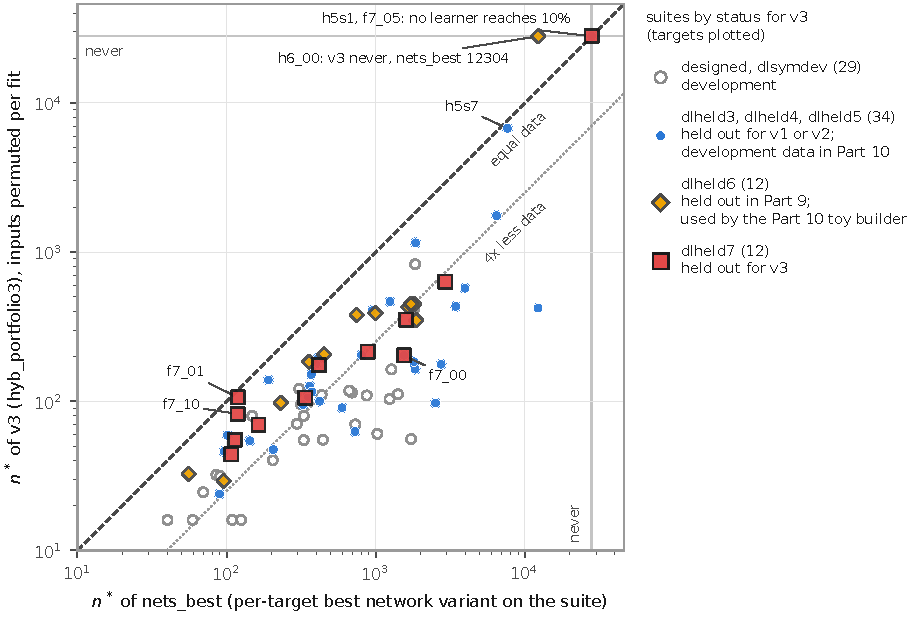
\includegraphics[width=\linewidth]{figures/fig_toy_nstar.pdf}
\caption{$\nstar$ of v3 (inputs permuted per fit) against \code{nets_best} for every target of every toy suite with network references, one point per target \status{Numerical}. Colour and shape give the status of the suite for v3 (\cref{tab:status}); the held-out suite \code{dlheld7} is drawn as large outlined squares. ``never'': 10\% error not reached by $n=16384$, drawn at the edge. Points below the dashed line need less data than the best network variant, and points below the dotted line at least $4\times$ less. \code{nets_best} is a minimum over 2 variants on \code{designed}, \code{random}, \code{dlheld} and \code{dlheld2}, 3 on \code{dlsymdev} and \code{dlheld3}--\code{dlheld5}, 5 on \code{dlheld6} and the 3 pre-registered ones on \code{dlheld7}. \code{dlfamdev} has no network runs and is not shown. Source: \repo{study/part10/LEARNER_RESULTS.json}.}
\label{fig:toy-nstar}
\end{figure}

\Cref{tab:toy-suites} summarizes all 11 suites, and \cref{fig:toy-nstar} shows every target with a network reference. \Cref{tab:status} gives each suite's status for v3: only \code{dlheld7} is held out, and the footnotes of \cref{tab:toy-suites} mark the suites that shaped v3 or an earlier version.

\paragraph{Results} \status{Numerical}. On the 126 targets of \cref{fig:toy-nstar}, v3 is clearly better than \code{nets_best} on 121 and needs at least $4\times$ less data on 54 (\texttt{figures/fig\_toy\_nstar.json}). Five targets are not wins:
\begin{itemize}
\item h6\_00 (\code{dlheld6}) is clearly worse: only the most regularized network learns it, at 12304;
\item f7\_01 (\code{dlheld7}) and h5s7 (\code{dlheld5}) are ties;
\item f7\_05 (\code{dlheld7}) and h5s1 (\code{dlheld5}) are learned by no learner.
\end{itemize}
\Cref{sec:res-toy-fail} discusses them. The suite means against \code{nets_best} range from $-1.50$ to $-2.44$ (\cref{tab:toy-suites}).

\paragraph{Against the one variant run on every suite} \status{Numerical}. The suite means against \code{nets_best} are not comparable across suites, because \code{nets_best} minimizes over different sets of variants. \code{nets_wd} is the one variant run on every suite with network results. Against it, v3's mean $\log_2\nstar$ ratio is:
\begin{itemize}
\item development suites: $-2.42$ on \code{designed} and $-2.53$ on \code{dlsymdev}; the Part 6 development check \code{random}: $-2.26$;
\item earlier held-out suites: $-2.03$ on \code{dlheld}, $-1.99$ on \code{dlheld2}, $-2.07$ on \code{dlheld3}, $-2.25$ on \code{dlheld4} and $-2.66$ on \code{dlheld5};
\item the two draws of the blind family: $-1.94$ on \code{dlheld6} and $-1.83$ on \code{dlheld7}.
\end{itemize}
The two draws of the blind family give the two smallest margins, but \code{dlheld2} is within 0.05 of \code{dlheld6}, and differences of this size on suites of 7 to 12 targets are within noise. If the gap is real, two explanations fit it, and the data do not separate them \status{Heuristic}. Several of the other suites informed the design of v3 or of an earlier version, so some selection in v3's favour is expected there. And the suites differ in kind: \code{dlheld}--\code{dlheld5} were written within the study, mostly from families close to its development targets, while the blind family was written by an agent that had not seen the sum-feature design.

\paragraph{Wins that need no feature search, over the held-out suites} \status{Numerical}. Excluding the 30 of the 77 targets of the seven held-out suites (\code{dlheld}--\code{dlheld7}) on which \code{lin} or \code{hgb} is already clearly better than \code{nets_best}, v3's mean against \code{nets_best} is $-2.11$ over the 44 that both learn, with 42 targets clearly better and 1 clearly worse (\texttt{figures/fig\_toy\_nstar.json}). The 30 are of two kinds: 6 halfspace-like targets on which \code{lin} wins (v3 is within the tie band of \code{lin} or below it on each), and 24, mostly formulas, decision lists, multiplexers and controls, on which \code{hgb} wins; \cref{app:further-toy} lists them. So the margins do not come from targets that are easy for trees or linear models. They come from the targets with parity or signed-sum structure, where both calibration references fail, and Part 8's ablations located the toy wins in DFG \cite{discretelearners2026}. The pooled summary over the seven held-out suites, most of them development data for v3, is in \cref{app:further-toy}.

% ------------------------------------------------------------------------------------------------------------------
\subsection{Where v3 is not better}\label{sec:res-toy-fail}

Five of the 126 targets with network references are not wins (\cref{fig:toy-nstar}).
\begin{itemize}
\item \emph{Learned by no learner.} f7\_05 $=[\tfrac12(s+14)\bmod3\ne0]$, $s=x_1+\dots+x_{14}$ (\code{dlheld7}), and h5s1, a signed 9-input count with accept set $\{-9,-5,-1,3,9\}$ times the parity $x_{10}x_{11}$ (\code{dlheld5}). No network variant, \code{lin} or \code{hgb} reaches 10\% error on either by $n=16384$ (3 seeds).
\item \emph{The one loss.} h6\_00, a residue class mod 3 of a 13-input count (\code{dlheld6}), is learned only by the most regularized network (\code{nets_cewd1.0}, $\nstar=12304$). It is the only target of any suite on which a network is clearly better than v3, and it was v2's loss as well. The third residue class mod 3, fd\_10 on 10 inputs (\code{dlfamdev}), has no network runs. v3 and v2 learn none of the three by $n=16384$.
\item \emph{Ties.} The halfspace f7\_01 $=[x_1+\dots+x_{13}\le1]$: v3 (106), \code{lin} (111) and the logistic-loss networks (119--121) are all within the tie band, and a linear readout of the inputs alone already does about as well. And h5s7, an arbitrary accept set of a signed 13-input count: 6760 against 7641 (\code{nets_cewd}).
\end{itemize}
The interpretability analysis (seed 0) locates the failures on the residue classes in DFG's search, not in its test: their true blocks would pass the test from $n=128$, but the targets have almost no Fourier weight at degrees 1--2, from which every seed of the search starts (\cref{sec:interp-toy-fail}; \cref{sec:dfg} explains why such a block is invisible to the seeds). h5s7 is a weaker case of the same mechanism, found at $n=8192$ on seed 0, and h5s1's bottleneck is detecting its modulating parity (\cref{app:interp-late}). The next-smallest margins are listed in \cref{app:further-toy}.

% ------------------------------------------------------------------------------------------------------------------
\subsection{Tabular data}\label{sec:res-tabular}

\paragraph{What v3 runs on tabular data.} DFG runs only when there are 2 classes and every column is binary or categorical ($\le256$ bits), and the image members only on images. So on 24 of the 26 datasets v3 runs v1's code, the stack of LightGBM, ExtraTrees, $k$-NN and logistic regression (its predictions were checked identical to v2's on one optdigits fit, and v2 runs v1's code path there), and its results there are v1's Part 8 result files. Only two datasets qualify for DFG: kr\_vs\_kp (development) and mushroom (Part 7 held-out set). On mushroom v3's own runs give v1's seed-mean errors at every $n$. On kr\_vs\_kp they differ from v1's at 3 of 4 sizes, but at no cell clearly (\cref{app:further-tab}).

\paragraph{What is held out.} HELDOUT2 (10 datasets) was fixed in a commit before any Part 8 design work (\texttt{04a215b2}). v1 was developed on the 5 development datasets only, and its code path has not changed since. HELDOUT2 contains no dataset on which DFG runs, so it is held out for this code path. The Part 7 held-out set is held out in the weaker sense that the Part 8 designers had read its MLP references. The 5 development datasets are in-sample.

\begin{table}[t]
\centering{\footnotesize\setlength{\tabcolsep}{4pt}
\begin{tabular}{llccc}
\toprule
split & reference & cells (better / tie / worse) & mean $\log_2$ ratio & datasets lower (sign test $p$)\\
\midrule
Part 7 held-out set & \code{mlp} & 59 (22/36/1) & $-0.331$ & 10 of 11 (0.012)\\
 & \code{mlp_reg} & 59 (16/40/3) & $-0.160$ & 9 of 11 (0.065)\\
 & \code{mlp_strong} & 54 (22/30/2) & $-0.339$ & 10 of 11 (0.012)\\
 & \code{mlp_best} & 59 (12/44/3) & $-0.114$ & 8 of 11 (0.23)\\
 & \code{hgb} & 59 (20/38/1) & $-0.259$ & 10 of 11 (0.012)\\
\midrule
Part 8 fresh set (HELDOUT2) & \code{mlp} & 53 (15/36/2) & $-0.445$ & 9 of 10 (0.021)\\
 & \code{mlp_reg} & 53 (16/35/2) & $-0.272$ & 8 of 10 (0.11)\\
 & \code{mlp_strong} & 53 (15/36/2) & $-0.284$ & 8 of 10 (0.11)\\
 & \code{mlp_best} & 53 (10/41/2) & $-0.168$ & 8 of 10 (0.11)\\
 & \code{hgb} & 53 (12/40/1) & $-0.250$ & 9 of 10 (0.021)\\
\midrule
development & \code{mlp} & 24 (4/20/0) & $-0.379$ & 5 of 5 (0.062)\\
 & \code{mlp_reg} & 24 (3/21/0) & $-0.267$ & 5 of 5 (0.062)\\
 & \code{mlp_best} & 24 (1/23/0) & $-0.244$ & 5 of 5 (0.062)\\
 & \code{hgb} & 24 (4/20/0) & $-0.270$ & 5 of 5 (0.062)\\
\bottomrule
\end{tabular}
}
\caption{v3 on the tabular datasets against the MLP references and \code{hgb} \status{Numerical}. ``Cells'': the $(\text{dataset},n)$ pairs compared, each a mean over 3 seeds, with the verdict rule of \cref{sec:metrics}. ``Mean $\log_2$ ratio'': of v3's test error to the reference's, over cells, errors floored at 0.002. The last column counts the datasets whose mean ratio over $n$ is below 0, with the two-sided sign-test $p$. \code{mlp_best} is the per-cell best of the Part 7--8 MLP variants (hindsight). \code{mlp_strong} was run on the Part 7 set only at $n\le10000$ (54 of 59 cells) and not on the development sets. On 24 of the 26 datasets v3's code path is v1's, so these are Part 8's numbers, except for v3's own runs on mushroom (identical errors) and kr\_vs\_kp. Source: \repo{study/part10/LEARNER_RESULTS.json}.}
\label{tab:real}
\end{table}

\paragraph{Results} (\cref{tab:real}) \status{Numerical}.
\begin{itemize}
\item \emph{HELDOUT2, against \code{mlp_best}:} mean $\log_2$ error ratio $-0.168$, a geometric-mean error about 11\% lower. 10 of 53 cells are better and 2 worse. The mean error is lower on 8 of 10 datasets, which is not significant (sign test $p=0.11$).
\item \emph{HELDOUT2, against single references:} the margins are larger: $-0.445$ against the baseline \code{mlp} (9 of 10 datasets, $p=0.021$), $-0.284$ against \code{mlp_strong} (8 of 10, $p=0.11$) and $-0.250$ against \code{hgb} (9 of 10, $p=0.021$).
\item \emph{The Part 7 set:} $-0.114$ against \code{mlp_best} (12 better, 3 worse, 8 of 11 datasets, $p=0.23$) and $-0.259$ against \code{hgb} (10 of 11, $p=0.012$).
\item \emph{Development:} $-0.244$ against \code{mlp_best}, lower on 5 of 5 ($p=0.062$).
\end{itemize}
The per-dataset picture is in \cref{app:further-tab}.

\paragraph{Where the tabular result comes from} \status{Heuristic}. The tabular numbers are those of a classical stack, and they say little about discrete feature search: in Part 8, DFG did not carry them, no single member family matched the stack, and default \code{hgb} alone did not beat the MLPs \cite{discretelearners2026} (\cref{app:further-tab}). This agrees with the tabular-learning literature. Tree ensembles tend to beat plain MLPs on medium-sized tabular data \cite{grinsztajn2022tree,shwartzziv2022tabular}. Stacking diverse models adds to that \cite{wolpert1992stacked,erickson2020autogluon}. And careful regularization and tuning of the MLP narrow the gap \cite{kadra2021welltuned,gorishniy2021revisiting}. The MLP references here are standard recipes without tabular-specific architectures, so the margins would likely shrink against a tuned tabular network \status{Heuristic}. The tabular evidence for v3 is therefore modest: it is not worse than the MLPs on average on fresh tabular data (2 of 10 datasets have higher mean error), it is better on average without statistical significance, and the reason is the classical stack, unchanged since Part 8.

\section{How well it does: images}\label{sec:results-img}

On images v3 runs its image members and the classical ones (\cref{tab:members}); DFG does not run. So on images v3 is v2 with one more member, \code{cgbt}, and a stacker refitted over all members (\cref{sec:image,sec:history}). This section gives v3's test error on the two QuickDraw sets held out for it (\cref{sec:res-img-heldout}) and on the image sets it was developed on (\cref{sec:res-img-dev}). It then asks where the gain over v2 comes from (\cref{sec:res-img-gain}) and what a fit costs (\cref{sec:res-img-compute}).

\paragraph{Sources and rules.} Errors and verdicts come from \repo{study/part10/LEARNER_RESULTS.json}, which \repo{study/part10/compare_learner.py} computes from the result files \texttt{<learner>\_\_<set>.json} in \repo{study/standard_tasks/results/}. Stacking weights, FLOPs and CPU seconds come from the same files and their \texttt{.info.json} records. The tables are generated by \texttt{make\_tables.py} and \cref{fig:images} by \texttt{make\_figures.py}.
\begin{itemize}
\item \emph{Which file is v3.} On \code{qd_c} and \code{qd_d} it is v3's own runs (\code{hyb_portfolio3}). On the development sets it is the frozen image candidate \code{p10_codes}, whose predictions on images are identical to v3's (checked at assembly, \repo{study/part10/hyb_portfolio3/ASSEMBLY.md}).
\item \emph{Cells and verdicts.} A cell is a (set, $n$) pair. The error is measured on the set's fixed 10000-point test set. v3 is \emph{better} or \emph{worse} than a reference at a cell when the errors differ by more than 10\% of the reference's error \emph{and} by more than 2 standard errors; otherwise the cell is a \emph{tie} (\cref{sec:metrics}).
\item \emph{Noise.} At $n=60000$ every learner ran seed 0 only. The standard error is then the test set's binomial noise alone, about 0.34 points at an error of 13\%, so 2 s.e.\ of a difference is about 1.0 point. The 10\% criterion asks for 1.3 points there, so it is the binding one.
\end{itemize}

% ------------------------------------------------------------------------------------------------------------------
\subsection{The held-out sets \code{qd_c} and \code{qd_d}}\label{sec:res-img-heldout}

\code{qd_c} and \code{qd_d} are ten fresh QuickDraw classes each (\cref{sec:tasks}). They were fixed in a commit before any Part 10 design work. No result of a Part 10 learner on them was read before v3 was frozen (\cref{sec:discipline}).
\begin{itemize}
\item \emph{Runs.} v3, v2, v1, \code{hgb}, \code{mlp_strong} and \code{mlp_wide} ran 3 seeds at $n=1000$ and $n=10000$ and seed 0 at $n=60000$. \code{mlp_xl} ran at $n=60000$ only. The control \code{mlp_pool} ran on \code{qd_c} at $n\in\{10000,60000\}$, seed 0. These are the pre-registered cells.
\item \emph{Where to look.} Panel (a) of \cref{tab:img-cells} gives every held-out cell, panel (a) of \cref{tab:img-summary} the verdicts, and \cref{fig:images} the learning curves.
\end{itemize}

\begin{table}[t]
\centering{\scriptsize\setlength{\tabcolsep}{3.4pt}\renewcommand{\arraystretch}{1.12}
\begin{tabular}{lrcccccccccc}
\toprule
set & $n$ & v3 & v2 & v1 & \code{hgb} & \hd{\code{mlp_}\\\code{strong}} & \hd{\code{mlp_}\\\code{wide}} & \hd{\code{mlp_}\\\code{xl}} & \hd{\code{mlp_}\\\code{best+}} & \hd{\code{mlp_}\\\code{pool}} & \code{cnn}\\
\midrule
\multicolumn{12}{l}{\emph{held out for v3 (Part 10): 3 seeds at $n\le10000$, seed 0 at $n=60000$}}\\
\code{qd_c} & 1000 & \textbf{26.58} & 27.48\rlap{$^{\circ}$} & 31.68 & 37.52 & 33.01 & 33.02 & -- & 33.01 & -- & 24.36\rlap{$^{\circ}$}\\
\code{qd_c} & 10000 & \textbf{16.17} & 17.79\rlap{$^{\circ}$} & 20.05 & 22.76 & 20.94 & 20.41 & -- & 20.41 & 19.37 & 14.84\rlap{$^{\circ}$}\\
\code{qd_c} & 60000 & \textbf{12.76} & 13.63\rlap{$^{\circ}$} & 15.77 & 18.22 & 16.08 & 14.12\rlap{$^{\circ}$} & 14.12\rlap{$^{\circ}$} & 14.12\rlap{$^{\circ}$} & 14.48 & --\\
\addlinespace[2pt]
\code{qd_d} & 1000 & \textbf{26.12} & 26.71\rlap{$^{\circ}$} & 30.21 & 35.33 & 31.62 & 31.40 & -- & 31.40 & -- & --\\
\code{qd_d} & 10000 & \textbf{16.38} & 17.82\rlap{$^{\circ}$} & 19.70 & 21.85 & 20.30 & 19.89 & -- & 19.89 & -- & --\\
\code{qd_d} & 60000 & \textbf{12.64} & 13.99\rlap{$^{\circ}$} & 15.97 & 17.48 & 15.34 & 14.31 & 13.83\rlap{$^{\circ}$} & 13.83\rlap{$^{\circ}$} & -- & --\\
\bottomrule
\end{tabular}
}
\caption{Test error (\%) on every image cell with a v3 result \status{Numerical}. Seed mean of 3 at $n\le10000$ and seed 0 at $n=60000$, except where a panel says otherwise. \code{mlp_xl}, \code{mlp_pool} and \code{cnn} are seed 0 everywhere. Bold: the lowest error among v3, v2, v1, \code{hgb}, \code{mlp_strong}, \code{mlp_wide} and \code{mlp_xl}. A reference's entry carries $^{\circ}$ where the cell is a tie with v3 and $^{\ast}$ where the reference is clearly better than v3. An unmarked entry is clearly worse than v3. ``--'': not run (yet). \code{mlp_best+} is the per-cell minimum over all MLP references, and it is defined only at the $n$ where the Part 7 \code{mlp} has run. \code{mlp_pool} is \code{mlp_strong} given v2's pooled sums (a control). \code{cnn} sees the unpermuted pixels (context, not a reference). Panel (b): v3 is seed 0 and the references are seed means. Panel (c): v3 and v2 are seed 0, and \code{mlp_strong}, \code{hgb} and v1 are seed means. ``Fashion'' is Fashion-MNIST. Source: \repo{study/part10/LEARNER_RESULTS.json}; markers by \code{compare_hybrid.cells}.}
\label{tab:img-cells}
\end{table}

\begin{table}[t]
\centering{\footnotesize\setlength{\tabcolsep}{5pt}
\begin{tabular}{llccc}
\toprule
sets & reference & $n$ & cells (better / tie / worse) & mean $\log_2$ ratio\\
\midrule
\code{qd_c}, \code{qd_d} & \code{mlp_strong} & all & 6 (6/0/0) & $-0.314$\\
 &  & $\le3000$ & 2 (2/0/0) & $-0.294$\\
 &  & $\ge10000$ & 4 (4/0/0) & $-0.324$\\
 & \code{mlp_wide} & all & 6 (5/1/0) & $-0.253$\\
 &  & $\le3000$ & 2 (2/0/0) & $-0.289$\\
 &  & $\ge10000$ & 4 (3/1/0) & $-0.235$\\
 & \code{mlp_xl} & all & 2 (0/2/0) & $-0.138$\\
 &  & $\ge10000$ & 2 (0/2/0) & $-0.138$\\
 & \code{mlp_best} & all & 2 (2/0/0) & $-0.343$\\
 &  & $\le3000$ & 1 (1/0/0) & $-0.313$\\
 &  & $\ge10000$ & 1 (1/0/0) & $-0.373$\\
 & \code{mlp_best+} & all & 2 (2/0/0) & $-0.325$\\
 &  & $\le3000$ & 1 (1/0/0) & $-0.313$\\
 &  & $\ge10000$ & 1 (1/0/0) & $-0.336$\\
 & v2 & all & 6 (0/6/0) & $-0.097$\\
 &  & $\le3000$ & 2 (0/2/0) & $-0.040$\\
 &  & $\ge10000$ & 4 (0/4/0) & $-0.125$\\
 & v1 & all & 3 (3/0/0) & $-0.271$\\
 &  & $\le3000$ & 1 (1/0/0) & $-0.210$\\
 &  & $\ge10000$ & 2 (2/0/0) & $-0.302$\\
 & \code{mlp_pool} (control) & all & 2 (2/0/0) & $-0.222$\\
 &  & $\ge10000$ & 2 (2/0/0) & $-0.222$\\
\midrule
\code{qd_a}, \code{qd_b}$^c$ & \code{mlp_strong} & all & 5 (5/0/0) & $-0.337$\\
 &  & $\le3000$ & 2 (2/0/0) & $-0.338$\\
 &  & $\ge10000$ & 3 (3/0/0) & $-0.337$\\
 & \code{mlp_wide} & all & 5 (5/0/0) & $-0.302$\\
 &  & $\le3000$ & 2 (2/0/0) & $-0.320$\\
 &  & $\ge10000$ & 3 (3/0/0) & $-0.291$\\
 & \code{mlp_xl} & all & 1 (1/0/0) & $-0.204$\\
 &  & $\ge10000$ & 1 (1/0/0) & $-0.204$\\
 & \code{mlp_best} & all & 5 (5/0/0) & $-0.337$\\
 &  & $\le3000$ & 2 (2/0/0) & $-0.338$\\
 &  & $\ge10000$ & 3 (3/0/0) & $-0.337$\\
 & \code{mlp_best+} & all & 5 (5/0/0) & $-0.294$\\
 &  & $\le3000$ & 2 (2/0/0) & $-0.320$\\
 &  & $\ge10000$ & 3 (3/0/0) & $-0.276$\\
 & \code{hgb} & all & 5 (5/0/0) & $-0.443$\\
 &  & $\le3000$ & 2 (2/0/0) & $-0.419$\\
 &  & $\ge10000$ & 3 (3/0/0) & $-0.460$\\
 & v2 & all & 5 (0/5/0) & $-0.089$\\
 &  & $\le3000$ & 2 (0/2/0) & $-0.064$\\
 &  & $\ge10000$ & 3 (0/3/0) & $-0.107$\\
 & v1 & all & 5 (5/0/0) & $-0.286$\\
 &  & $\le3000$ & 2 (2/0/0) & $-0.246$\\
 &  & $\ge10000$ & 3 (3/0/0) & $-0.314$\\
 & \code{mlp_pool} (control) & all & 3 (3/0/0) & $-0.204$\\
 &  & $\ge10000$ & 3 (3/0/0) & $-0.204$\\
 & \code{cnn} (context) & all & 1 (0/0/1) & $+0.245$\\
 &  & $\ge10000$ & 1 (0/0/1) & $+0.245$\\
\bottomrule
\end{tabular}
}
\caption{v3 against each image reference \status{Numerical}. ``Cells'' counts the (set, $n$) pairs compared, with v3 better / tied / worse by the cell rule (\cref{sec:metrics}). ``Mean $\log_2$ ratio'' is the mean over those cells of $\log_2$(v3's error / the reference's error); negative means v3 is lower. \code{mlp_best} is the per-cell minimum over the Part 7--8 MLP variants (\code{mlp}, its regularized versions, \code{mlp_strong} and its single network \code{mlp_strong1}). \code{mlp_best+} adds \code{mlp_wide}, its single network \code{mlp_wide1}, and \code{mlp_xl}. Both are defined only where the Part 7 \code{mlp} has run. Panels (b) and (c) compare single v3 fits (seed 0) with the references' seed means. Source: \repo{study/part10/LEARNER_RESULTS.json}.}
\label{tab:img-summary}
\end{table}

\begin{figure}[tbp]
\centering
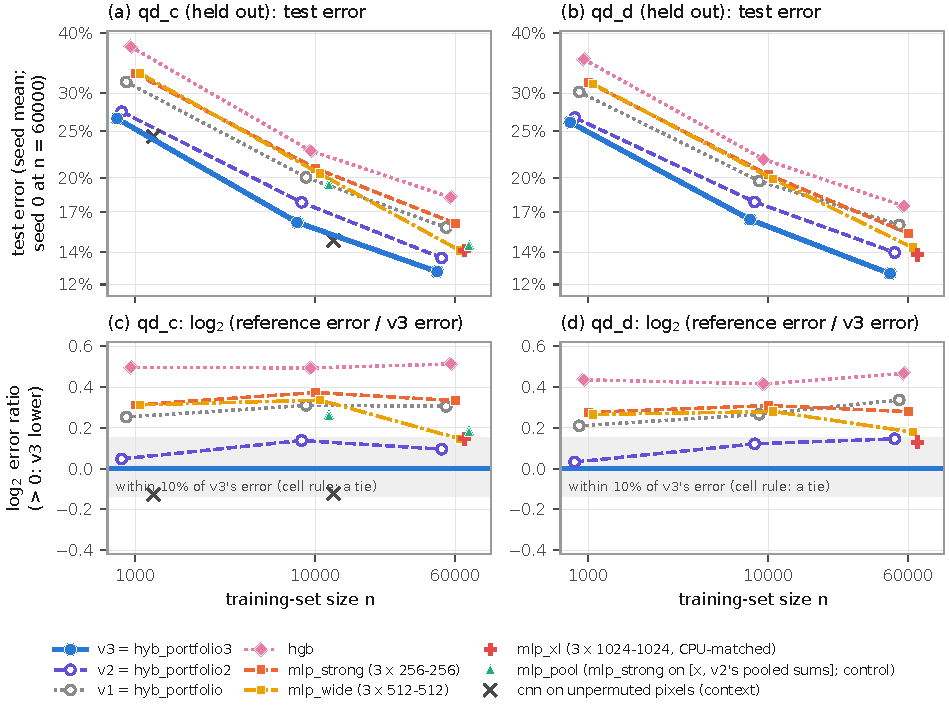
\includegraphics[width=\textwidth]{figures/fig_images.pdf}
\caption{The held-out QuickDraw sets \status{Numerical}. Top: test error against $n$ (log--log; seed mean of 3 at $n\le10000$, seed 0 at $n=60000$; \code{mlp_xl}, \code{mlp_pool} and \code{cnn} seed 0). Bottom: each reference's error relative to v3's at the same $n$, as $\log_2$(reference error / v3 error), so points above 0 are cells where v3 is lower. In the grey band the two errors are within 10\% of each other, and the cell rule calls the cell a tie whatever the noise. Markers are shifted slightly sideways so that they do not hide each other. Generated by \texttt{make\_figures.py} (\texttt{fig\_images}) from the result files; the plotted values are in \texttt{figures/fig\_images.json}.}
\label{fig:images}
\end{figure}

\paragraph{Against the MLP references} \status{Numerical}. At all six held-out cells v3's error is lower than every reference's and the control's.
\begin{itemize}
\item \code{mlp_strong} (ensemble of three 256-256 networks): v3 is clearly better at all 6 cells. Its error is 17--23\% lower, and the mean $\log_2$ ratio is $-0.31$ ($-0.32$ at $n\ge10000$).
\item \code{mlp_wide} (three 512-512 networks): clearly better at 5 cells. The sixth, \code{qd_c} at $n=60000$, is a tie: 12.76\% against 14.12\%, 9.6\% lower, just inside the 10\% threshold. Mean $-0.25$.
\item \code{mlp_xl} (three 1024-1024 networks, the CPU-matched reference; $n=60000$ only): two ties. v3 is 9.6\% lower on \code{qd_c} (12.76\% against 14.12\%) and 8.6\% lower on \code{qd_d} (12.64\% against 13.83\%). Mean $-0.14$.
\item \code{mlp_best} and \code{mlp_best+} are defined so far only on \code{qd_c} at $n=1000$ and $n=10000$, because the Part 7 \code{mlp} has run only up to $n=10000$ there. v3 is clearly better at both cells.
\end{itemize}
\todo{The Part 7 mlp on qd\_c ($n\ge30000$) and on qd\_d is still running. When it lands, mlp\_best and mlp\_best+ cover more cells: update this item and panel (a) of the summary table.}

So at $n\le10000$ v3 is clearly better than every MLP reference. At $n=60000$ the two widest ensembles come within 10\% of it on \code{qd_c}, and \code{mlp_xl} also on \code{qd_d}.

\paragraph{Against the other references} \status{Numerical}.
\begin{itemize}
\item \code{hgb} (on \code{qd_c} so far): v3 is clearly better at all 3 cells, with errors 29--30\% lower (mean $\log_2$ ratio $-0.50$).
\item v1, the Part 8 portfolio (on \code{qd_d} so far): clearly better at all 3 cells, by 13.5\%, 16.9\% and 20.9\% at $n=1000$, 10000 and 60000.
\item v2: all 6 cells are ties. v3's error is lower at every cell, by 2.2--3.3\% at $n=1000$ and by 6.4--9.6\% at $n\ge10000$, but never by more than 10\%. The mean $\log_2$ ratio is $-0.10$, and $-0.125$ at $n\ge10000$.
\end{itemize}
\todo{hgb on qd\_d and v1 on qd\_c are still running. When they land, update these two items (counts and ranges) and the summary table.}

\paragraph{The control and the context} \status{Numerical}.
\begin{itemize}
\item \code{mlp_pool} is \code{mlp_strong} given v2's pooled subset sums as extra inputs (seed 0, \code{qd_c} only). v3 is clearly better at both cells: 16.17\% against 19.37\% at $n=10000$, and 12.76\% against 14.48\% at $n=60000$. v2 ties it at both cells (17.79\% and 13.63\%, which are 8.2\% and 5.9\% lower), as it did on \code{qd_a} and \code{qd_b} in Part 9. This control matches v2's representation, not v3's: no MLP was given the bar sums (\cref{sec:res-img-gain}).
\item \code{cnn}, a small convolutional network on the unpermuted pixels, is context, not a reference. Its \code{qd_c} runs ($n=1000$ and 10000) are still in progress.
\end{itemize}
\todo{cnn on qd\_c is running: add its two cells here and in the tables (context only; on qd\_a at $n=10000$ it was better than v3, \cref{sec:res-img-dev}).}

\paragraph{The best-learner rule}\label{sec:res-img-rule} \status{Numerical}. The pre-registered rule does not use cell verdicts (\cref{sec:discipline}). It makes v3 the learner of this paper if two conditions hold:
\begin{itemize}
\item the mean $\log_2$ error ratio of v3 to v2 over the four held-out image cells with $n\ge10000$ is below 0. It is $-0.125$: the cells give $-0.138$ and $-0.095$ on \code{qd_c} ($n=10000$, 60000) and $-0.122$ and $-0.146$ on \code{qd_d};
\item the mean $\log_2\nstar$ ratio of v3 to v2 on \code{dlheld7} is at most $+0.1$. It is $-0.004$ (\cref{sec:res-dlheld7}).
\end{itemize}
Both hold, so v3 replaced v2. The rule was applied by \repo{study/part10/compare_part10.py} (\repo{study/part10/RESULTS.md}) after every held-out cell of v3 and v2 was in, and the decision is recorded in \repo{study/part10/PROTOCOL.md} (28 October, 04:25 UTC).

\paragraph{How firm the gain over v2 is.} By the cell rule it is not established at any single cell. Its direction is consistent: in all 14 seed-paired fits (same training sample, same test set), v3's error is below v2's, by 0.47 to 1.86 points \status{Numerical}. This is a description made after the results were in, not a pre-registered test. The 14 fits share two test sets, so they are not independent.

% ------------------------------------------------------------------------------------------------------------------
\subsection{The other image sets: development data for v3}\label{sec:res-img-dev}

Panels (b) and (c) of \cref{tab:img-cells,tab:img-summary} give v3 at the cells of its fixed development evaluation. These sets are not held out for v3, and the cells are in-sample for a choice:
\begin{itemize}
\item \emph{Tuning.} The image builders tuned on validation rows of the training pools of \code{qd_dev}, \code{qd_a} and Fashion-MNIST, never on a test set. \code{qd_b} was not used in \code{p10_codes}'s development (\repo{study/part10/p10_codes/DESIGN.md}).
\item \emph{Selection.} After each freeze, the candidate's test error was computed once at 8 cells: \code{qd_dev} and Fashion-MNIST at $n\in\{1000,10000\}$, and \code{qd_a} and \code{qd_b} at $n\in\{3000,10000\}$. A ninth cell, \code{qd_a} at $n=60000$, was added as a check. The integration rule then used these test errors to qualify the two candidates and choose between them (\repo{study/part10/RESULTS.md}).
\item \emph{The choice.} \code{p10_codes} had a mean $\log_2$ ratio against v2 of $-0.078$ over the 8 cells, and at \code{qd_a}, $n=60000$, 10.82\% error, 1453 CPU s and 0.58 of the FLOP budget. \code{p10_hier} had $-0.071$, 11.08\%, 924 s and 0.44. The rule took the lower mean.
\end{itemize}
The v3 numbers here are therefore the errors of the candidate that these very numbers selected. With two candidates this close the selection effect is small, but these cells are not a test of v3. Each v3 entry is one fit (seed 0).

\paragraph{\code{qd_a} and \code{qd_b}} (held out in Part 9) \status{Numerical}.
\begin{itemize}
\item \emph{References.} v3 is clearly better than \code{mlp_strong}, \code{mlp_wide}, \code{hgb} and v1 at all 5 cells. It is also clearly better than \code{mlp_xl} at \code{qd_a}, $n=60000$ (10.82\% against 12.46\%, 13.2\% lower), and than \code{mlp_pool} at the 3 cells where both were run (at \code{qd_a}, $n=60000$: 10.82\% against 12.25\%).
\item \emph{v2.} All 5 cells are ties, with v3 2.6--9.6\% lower (mean $\log_2$ ratio $-0.089$). Here v2's entries are seed means. Against v2's seed-0 fits, as the integration rule compared them, the margins are similar: for example 17.48\% against 18.75\% at \code{qd_a}, $n=3000$.
\item \emph{The context.} The \code{cnn} on unpermuted pixels is the only learner better than v3: 12.00\% against 14.22\% at \code{qd_a}, $n=10000$, an error 18.5\% lower. Among v3's cells, only the one at $n=60000$ (10.82\%) is below it.
\item \emph{Comparison with Part 9.} At $n=60000$, v2 tied \code{mlp_xl} on both sets (11.97\% against 12.46\% on \code{qd_a}; 14.88\% against 14.79\% on \code{qd_b}). The control \code{mlp_pool} matched v2 (12.25\% and 14.74\%). v3's \code{qd_a} cell (10.82\%) is clearly better than both. v3 was not run at \code{qd_b}, $n=60000$.
\end{itemize}

\paragraph{\code{qd_dev} and Fashion-MNIST} (development throughout) \status{Numerical}.
\begin{itemize}
\item \emph{\code{qd_dev}.} v3 is clearly better than \code{mlp_strong}, \code{hgb} and v1 at both cells, for example 13.30\% against \code{mlp_strong}'s 17.49\% at $n=10000$. It ties v2 at both cells (21.18\% against 22.22\%, 13.30\% against 14.63\%).
\item \emph{Fashion-MNIST.} Every comparison is a tie. v3 has 17.97\% and 12.38\% against \code{mlp_strong}'s 18.60\% and 12.64\% (3.4\% and 2.0\% lower). It also ties v2, v1 and \code{hgb}. This is the set where the bars do not help. On the builder's validation rows, a booster on \code{cgbt}'s bank was worse there than one on v2's bank (18.30\% against 17.74\% at $n=1000$; \repo{study/part10/p10_codes/DESIGN.md}, \S4.2). \code{cgbt}'s stacking weight is 0.05 and 0.07 there, against 0.23--0.50 on the QuickDraw development cells.
\item \emph{Larger $n$.} v3 was not run on Fashion-MNIST beyond $n=10000$. v2's image path (\code{p9_gates}, Part 9, seed 0) reached 9.64\% at $n=60000$, against \code{mlp_strong}'s 9.66\%.
\item \emph{A threading caveat.} v2's own cells on these two sets were run with multi-threaded BLAS, while every v3 and held-out run is single-threaded. A single-threaded refit of v2 at \code{qd_dev}, $n=10000$, gives 14.67\% instead of 14.63\% (\repo{study/part10/PROTOCOL.md}, note).
\end{itemize}

% ------------------------------------------------------------------------------------------------------------------
\subsection{Where the gain over v2 comes from}\label{sec:res-img-gain}

\begin{table}[t]
\centering{\scriptsize\setlength{\tabcolsep}{3.3pt}
\begin{tabular}{lrccccccccccccc}
\toprule
 & & \multicolumn{5}{c}{v3: stacking weight} & \multicolumn{4}{c}{v2: stacking weight} & \multicolumn{4}{c}{out-of-fold error (\%)}\\
\cmidrule(lr){3-7}\cmidrule(lr){8-11}\cmidrule(lr){12-15}
set & $n$ & \code{cgbt} & \code{ggbt} & \code{gknn} & \code{knn} & rest & \code{ggbt} & \code{gknn} & \code{knn} & rest & \code{cgbt} & \code{ggbt} & v3 & v2\\
\midrule
\code{qd_c} & 1000 & 0.27 & 0.02 & 0.38 & 0.15 & 0.03 & 0.24 & 0.46 & 0.17 & 0.04 & 30.8 & 32.5 & 27.6 & 29.0\\
\code{qd_c} & 10000 & 0.36 & 0.04 & 0.15 & 0.15 & 0.01 & 0.35 & 0.24 & 0.18 & 0.03 & 16.8 & 18.9 & 16.2 & 17.2\\
\code{qd_c} & 60000 & 0.49 & 0.12 & 0.11 & 0.17 & 0.00 & 0.50 & 0.20 & 0.24 & 0.00 & 13.3 & 14.6 & 12.8 & 13.5\\
\code{qd_d} & 1000 & 0.23 & 0.08 & 0.30 & 0.18 & 0.03 & 0.27 & 0.35 & 0.21 & 0.04 & 28.1 & 29.8 & 26.3 & 26.1\\
\code{qd_d} & 10000 & 0.39 & 0.01 & 0.13 & 0.19 & 0.01 & 0.29 & 0.20 & 0.26 & 0.10 & 17.1 & 19.2 & 16.2 & 17.3\\
\code{qd_d} & 60000 & 0.45 & 0.12 & 0.04 & 0.12 & 0.00 & 0.50 & 0.11 & 0.23 & 0.00 & 12.6 & 14.3 & 12.5 & 13.5\\
\bottomrule
\end{tabular}
}
\caption{What carries v3 and v2 on the held-out image sets \status{Numerical}. Left: stacking weight per member family (seed mean of 3 fits at $n\le10000$; one fit at $n=60000$). \code{gknn}: $k$-NN votes on the pooled sums. \code{knn}: $k$-NN votes on the pixels. ``rest'': Part 8's \code{gbt}, \code{et} and \code{lin}; \code{lin} has weight 0 in every fit here. Right: out-of-fold error on the training rows of the two boosters and of the whole stack (5-fold at $n\le3000$; one holdout of 2000 rows at $n=10000$ and 6000 rows at $n=60000$). \code{ggbt}'s out-of-fold error is the same in v3 and v2 in every fit. The weights multiply log-probabilities of different calibration, so they are not shares of the decision. Source: \texttt{hyb\_portfolio\{3,2\}\_\_qd\_\{c,d\}.info.json} in \repo{study/standard_tasks/results/}.}
\label{tab:img-stack}
\end{table}

\paragraph{The same members, plus one} \status{Numerical}. In each of the 14 held-out fits, v3's and v2's records give every shared member the same out-of-fold error, and \code{ggbt} the same number of boosting rounds. \code{cgbt} draws from its own random stream, so v3's other members are v2's fits. v3 and v2 therefore differ only by \code{cgbt} and by the stacking weights. The final refits also differ where a weight moves between zero and a positive value, because a member with weight 0 is not refitted. \Cref{tab:img-stack} gives the weights and the out-of-fold errors.
\begin{itemize}
\item \emph{\code{cgbt} is the better booster.} Its out-of-fold error is below \code{ggbt}'s in all 14 fits: by 0.2--4.0 points at $n=1000$, and by 0.13--0.20 in $\log_2$ at $n\ge10000$. It is the lowest of all members in 13 of the 14 fits. The exception is \code{qd_c}, $n=1000$, seed 1, where $k$-NN on pooled sums is lower (30.1\% against 31.8\%).
\item \emph{It takes \code{ggbt}'s place in the stack.} At $n\ge10000$, \code{cgbt} has the largest family weight in all 8 fits (0.32--0.49). \code{ggbt}'s weight falls from 0.25--0.50 in v2 to 0--0.12 in v3. At $n=1000$, the $k$-NN votes on pooled sums keep the largest family weight in 5 of 6 fits, in v3 as in v2.
\item \emph{The stack improves.} v3's stacked out-of-fold error is below v2's in 12 of the 14 fits. At \code{qd_d}, $n=1000$, it is equal in one fit and higher in one (27.2\% against 26.3\%).
\end{itemize}
Two cautions about the weights apply (\cref{sec:interp-img}). They multiply log-probabilities of different calibration: boosters stopped early on error are over-confident, while $k$-NN votes are smooth. And the convex stacker splits weight between two nearly collinear boosters on one holdout. So ``\code{ggbt} gets weight 0'' describes one fit, not a property of the learner.

\paragraph{What \code{cgbt} changes: the bank, not the schedule} \status{Numerical}. \code{cgbt} has \code{ggbt}'s tree settings and early-stopping rule. It differs from \code{ggbt} in three ways: its bank adds bar sums at two lengths, it drops the 300 prototype-pair projections, and its per-tree column fraction is 0.05 instead of 0.12 (\cref{sec:image}). The builder's development runs separate these effects (one booster alone, $n=5000$, validation rows, seed 0; \repo{study/part10/p10_codes/DESIGN.md}, \S4.2). On \code{qd_dev}:
\begin{itemize}
\item v2's bank gave 17.66\% error, and dropping the pairs gave 17.20\%;
\item adding the bars at both lengths gave 15.92\%, and the lower column fraction then gave 15.82\%.
\end{itemize}
On \code{qd_a} the full change gave 17.68\% $\to$ 16.78\%. So on QuickDraw most of the gain is the bars. On Fashion-MNIST the bars did not help. In \code{cgbt}'s fitted trees the bars, two thirds of its columns, carry 0.72--0.80 of the split gain on QuickDraw and MNIST (development fits; \cref{sec:interp-img}). Split gain describes how the trees split, not what the predictions depend on.

\paragraph{Compared with Part 9} \status{Numerical}. In Part 9, at $n=60000$ on \code{qd_a} and \code{qd_b}, v2 tied the CPU-matched \code{mlp_xl}, and the control \code{mlp_pool} matched v2. Most of v2's large-$n$ advantage over the MLPs was therefore the pooled-sum representation, which an MLP uses as well as the trees do. The Part 10 held-out sets repeat this for v2:
\begin{itemize}
\item v2 ties \code{mlp_xl} at $n=60000$ on both sets (13.63\% against 14.12\%; 13.99\% against 13.83\%);
\item v2 ties \code{mlp_pool} at both \code{qd_c} cells.
\end{itemize}
v3 moves past the control: it is clearly better than \code{mlp_pool} at both cells, by 16.5\% and 11.9\%. Against \code{mlp_xl} it is 9.6\% and 8.6\% lower, just inside the 10\% threshold.

\paragraph{Reading} \status{Heuristic}. On images v3's gain over v2 is a better fixed representation for gradient-boosted trees: sums over short runs of pixels along lines recovered from pixel correlations, used at fixed positions. Recovering the image topology from such correlations is an old idea \cite{leroux2007topology}, and so is grouping inputs into receptive fields by their correlations \cite{coates2011receptive}. The gain is not evidence that discrete search beats gradient-based learning on images, for three reasons.
\begin{itemize}
\item \emph{The control for v3's own representation was not run.} No MLP was given the bar sums as well as the pooled sums. Part 9's control matched v2 once it had v2's features, so part of v3's margin over the MLPs may again be available to a network given the same features.
\item \emph{Gradient-trained networks that learn local structure were not run.} For example, an MLP trained to learn sparse local connectivity \cite{neyshabur2020convolutions} would be the information-matched comparison.
\item \emph{A network told the layout is better.} At the one cell where both have run, the small \code{cnn} has 12.00\% error against v3's 14.22\% (\code{qd_a}, $n=10000$).
\end{itemize}
What v3 shows is narrower: a learner that never reads the pixel layout, and whose features are fixed subset sums chosen by rank statistics, reaches 12.6--12.8\% error on fresh QuickDraw classes at $n=60000$. That is 8.6--9.6\% below a CPU-matched MLP ensemble, a tie by the cell rule, and clearly below an MLP given v2's representation (\code{qd_c}).

% ------------------------------------------------------------------------------------------------------------------
\subsection{Compute}\label{sec:res-img-compute}

\begin{table}[t]
\centering{\scriptsize\setlength{\tabcolsep}{3.2pt}
\begin{tabular}{lrccccccccc}
\toprule
 & & \multicolumn{2}{c}{FLOPs / budget} & \multicolumn{3}{c}{CPU s per fit} & \multicolumn{4}{c}{MLP references: wall s per fit (FLOPs / budget)}\\
\cmidrule(lr){3-4}\cmidrule(lr){5-7}\cmidrule(lr){8-11}
set & $n$ & v3 & v2 & v3 & \hd{of which\\\code{cgbt}} & v2 & \code{mlp_strong} & \code{mlp_wide} & \code{mlp_xl} & \code{mlp_pool}\\
\midrule
\code{qd_c} & 1000 & 0.49--0.51 & 0.35 & 229--256 & 120--132 & 144--166 & 384 (2.0) & 249 (5.0) & -- & --\\
\code{qd_c} & 10000 & 0.34--0.48 & 0.22--0.26 & 513--785 & 251--430 & 284--440 & 490 (2.0) & 396 (5.0) & -- & 333 (5.9)\\
\code{qd_c} & 60000 & 0.57 & 0.42 & 1361 & 668 & 1296 & 963 (2.0) & 1168 (5.0) & 2196 (9.2) & 716 (5.9)\\
\addlinespace[2pt]
\code{qd_d} & 1000 & 0.50--0.51 & 0.35 & 266--291 & 128--140 & 162--175 & 98 (2.0) & 248 (5.0) & -- & --\\
\code{qd_d} & 10000 & 0.30--0.46 & 0.24--0.29 & 402--768 & 233--377 & 394--602 & 152 (2.0) & 440 (5.0) & -- & --\\
\code{qd_d} & 60000 & 0.58 & 0.42 & 1464 & 760 & 1531 & 422 (2.0) & 989 (5.0) & 1335 (9.2) & --\\
\bottomrule
\end{tabular}
}
\caption{Compute per fit on the held-out image cells \status{Numerical}. Budget: three training runs of the baseline MLP (\code{common.budget_real}), $1.24$, $2.42$ and $6.21\times10^{12}$ FLOPs at $n=1000$, 10000 and 60000. FLOPs / budget: each learner's own count, everything in the fit included and prediction excluded. CPU s: process CPU seconds per fit, and the seconds v3 attributes to \code{cgbt}. A range is over the 3 seeds; $n=60000$ has one fit. The MLP references record wall-clock seconds per fit on the shared 4-core machine, not process CPU time (the \texttt{cpu\_seconds} field of their result files), with their FLOPs per fit in units of the budget in brackets. Sources: the result files and \texttt{.info.json} records in \repo{study/standard_tasks/results/}.}
\label{tab:img-compute}
\end{table}

\paragraph{FLOPs} \status{Numerical}. The budget of a real-data fit is three training runs of the baseline MLP: $1.24\times10^{12}$ FLOPs at $n=1000$, $2.42\times10^{12}$ at $n=10000$ and $6.21\times10^{12}$ at $n=60000$ (\cref{tab:img-compute}).
\begin{itemize}
\item \emph{v3 and v2.} By its own count v3 uses 0.30--0.58 of the budget on the held-out cells, the most at $n=60000$. v2 uses 0.22--0.42. \code{cgbt} adds 0.05--0.22.
\item \emph{Near the guard at $n=3000$.} On the development sets, at $n=3000$ (no held-out cell has this size), v3 used 0.85 of the budget on \code{qd_a} and on \code{qd_b}. That is close to the guard at 0.9, which skips members whose projected cost would exceed it (\cref{sec:portfolio}). Part 9's compute audit found that the FLOP charge of Part 8's \code{gbt} member is too low by a factor of 1.14--1.46 at this size, and it projected v2's $n=3000$ QuickDraw cells at about 0.72 (0.69--0.81) of the budget, against v2's own count of at most 0.62. v3 keeps that charge, and no compute audit was made of v3. Applying the audit's factor to \code{gbt} alone (0.28 of the budget by v3's count) puts these two cells at 0.88--0.98 \status{Heuristic}. So v3 is within the budget at $n=3000$ by its own count, but not with a clear margin.
\item \emph{The MLP references.} Every MLP reference spends more FLOPs than the budget: \code{mlp_strong} 2.0 budgets per fit (six training runs), \code{mlp_wide} 5.0, \code{mlp_pool} 5.9 and \code{mlp_xl} 9.2. So by FLOPs v3 is cheaper than every MLP reference at every cell, by a factor of at least 3.4 (\code{mlp_strong} at \code{qd_d}, $n=60000$).
\end{itemize}

\paragraph{CPU time} \status{Numerical}. Equal FLOPs are far from equal CPU time.
\begin{itemize}
\item \emph{v3 and v2.} A v3 fit takes 229--291 CPU s at $n=1000$, 402--785 s at $n=10000$, and 1361 and 1464 s at $n=60000$. v2 takes 144--175, 284--602, and 1296 and 1531 s.
\item \emph{Why v3 is not slower at $n=60000$.} There v3 takes about as long as v2 (1.05$\times$ on \code{qd_c}, 0.96$\times$ on \code{qd_d}), although it fits a second booster. \code{cgbt} takes 668 and 760 s. But v3's \code{ggbt} takes 482 and 474 s against v2's 1091 and 1305 s. The reason is that v3 sets LightGBM's column-wise layout, which leaves the predictions unchanged (\repo{study/part10/p10_codes/DESIGN.md}, \S1). Part 9 found this fix but did not apply it to v2.
\item \emph{A like-for-like estimate.} The comparison with v2 is not like for like. v3's time minus \code{cgbt}'s, 693 and 704 s, estimates v2 with the same layout. By that estimate the second booster about doubles the CPU time of a fit at $n=60000$.
\item \emph{The MLP references.} At $n=60000$ they take 963 and 422 s of wall time (\code{mlp_strong}), 1168 and 989 s (\code{mlp_wide}) and 2196 and 1335 s (\code{mlp_xl}); \code{mlp_pool} takes 716 s. So \code{mlp_xl} takes about as long as v3, which is the sense in which it is CPU-matched. The other ensembles take 0.3--0.9 of v3's time.
\item \emph{How rough the MLP times are.} They are wall-clock seconds on the shared machine, and they vary with the load from concurrent jobs. The same \code{mlp_strong} recipe took 384 s per fit at \code{qd_c}, $n=1000$, and 98 s at \code{qd_d}, $n=1000$. In Part 9 it took 28 s at \code{qd_a}.
\end{itemize}

\paragraph{Prediction} is not charged for any learner. A v2 query costs about $2.8\times10^8$ FLOPs at $n=60000$, about $500\times$ an MLP's, because the $k$-NN members scan the training set (Part 9). v3 adds \code{cgbt}'s bank projection, about $1.2\times10^7$ FLOPs per query, and up to about 4000 more tree traversals (\repo{study/part10/p10_codes/DESIGN.md}, \S6).

% ------------------------------------------------------------------------------------------------------------------
\paragraph{Summary of the image results.}
\begin{itemize}
\item \emph{Strong points} \status{Numerical}. On the two held-out sets v3 is clearly better than \code{mlp_strong} at every cell, and than every MLP reference at $n\le10000$. It is clearly better than the control \code{mlp_pool} at both cells where that was run. Its error is below every reference's at every held-out cell.
\item \emph{Weak points} \status{Numerical}. At $n=60000$ the CPU-matched \code{mlp_xl} is within 10\% of v3 on both sets (two ties), and \code{mlp_wide} on \code{qd_c}. v3's gain over v2 is below the cell rule's threshold at every cell; the best-learner rule, which uses mean $\log_2$ ratios, still prefers v3. On Fashion-MNIST v3 is level with \code{mlp_strong}. The \code{cnn} that sees the layout is better at the one cell where both have run. A fit takes 23--24 CPU minutes at $n=60000$. The FLOP count reaches 0.85 of the budget at $n=3000$, and with Part 9's audited correction it would be close to 1.
\item \emph{What it means} \status{Heuristic}. The gain over v2 comes from a richer fixed feature bank for gradient-boosted trees, not from a new kind of learning. Whether an MLP would gain as much from the same bank was not tested.
\end{itemize}

\section{What it learns}\label{sec:interp}

This section describes what v3's fitted members contain on the toy targets (\cref{sec:interp-toy}) and on images (\cref{sec:interp-img}). The analysis is descriptive: it says what structure the fits hold and when it appears, not why v3 does well, and nothing here is an ablation of the learner or a causal test. Every analysed fit is an instrumented seed-0 rerun of an evaluation fit, with the same training rows, column permutation and random streams. On the toy side every rerun reproduces the evaluation's seed-0 test error; on images, every rerun that has an evaluation cell reproduces it (\cref{app:interp-workflow}). Two independent verifiers per side checked the numbers and the readings, and their corrections are used throughout. Measured quantities are \status{Numerical}; descriptions of maps and explanations of mechanisms are \status{Heuristic}.

\paragraph{Findings.}
\begin{enumerate}
\item \emph{DFG finds the exact signed blocks} on 49 of the 54 sum-structured targets (median $n_{\rm struct}=256$), and its mean output then follows $E[f\mid t]$ level by level (\cref{sec:interp-toy-struct}).
\item \emph{Detection is cheap; discovery lags.} On the 25 pure symmetric targets the true block would pass DFG's test at $n=128$ every time. The delay to discovery tracks the share of variance at Fourier degrees 1--2 (Spearman $-0.86$), and the 10\% error point arrives with the block (\cref{sec:interp-toy-timing}). Since every seed of the block search starts from those statistics, this reads as the search, not the test, setting DFG's data cost \status{Heuristic}.
\item \emph{The residue classes mod 3 are never proposed.} They have $W_1+W_2\le0.0002$; the search's orders reach their block no better than chance and no piece of it carries signal, although at $n=16384$ the true block would pass the test at 134--155 times the threshold (\cref{sec:interp-toy-fail}).
\item \emph{Pooling sets and bars recover local pieces of the pixel grid.} On QuickDraw 98.3--99.9\% of the other members of a 4-pixel set lie within one step, and bars are short runs along recovered lines; on Fashion-MNIST 7\% of the 4-pixel sets include the mirror pixel (\cref{sec:interp-img-geom}).
\item \emph{The bar booster carries v3 on QuickDraw and MNIST.} \code{cgbt} has the lowest out-of-fold error of all 18 members in every analysed fit and takes \code{ggbt}'s stacking weight there; bars carry 0.77--0.80 of its split gain, 1.1--1.2 times their column share (\cref{sec:interp-img-members}).
\item \emph{Much class evidence lies on blank pixels}: 0.56--0.69 of \code{cgbt}'s net TreeSHAP evidence, often where other classes have ink, though per pixel inked pixels carry more on QuickDraw and MNIST (\cref{sec:interp-img-maps}).
\end{enumerate}
\Cref{app:interp-detail} has the per-target detail, the models below the discovery size and on the other suites, and the caveats; \cref{app:further-v2v3} says where v1.3's additions act in the fitted models.

% ==================================================================================================================
\subsection{Toy targets: the search, not the test, sets DFG's data cost}\label{sec:interp-toy}

On toy inputs v3 is a stack of DFG v1.3 (a default variant and, at $n\le512$, a forced small-$n$ variant) and the classical members (\cref{sec:portfolio}). The analysis looks at DFG's final model in each fit. It covers the 54 sum-structured targets of the six suites built around signed sums (\code{dlsymdev}, \code{dlfamdev}, \code{dlheld4}--\code{dlheld7}; the 14 non-symmetric controls are excluded) and, more briefly, the 70 targets of the other suites. The grid is $n=16,32,\dots,16384$, stopped after two consecutive sizes with test error $\le0.005$.

\paragraph{Definitions.}
\begin{itemize}
\item \emph{Terms and shares.} The model's terms are its characters, sum blocks (\cref{sec:dfg}), spectral features and the kernel background. A term's \emph{share} is the standard deviation of its contribution to the model's output over the 4096 test inputs.
\item \emph{Exact structure.} The target's signed-symmetry classes are the sets of inputs it treats alike, up to sign. A class of size $\ge3$ is \emph{matched exactly} when a sum block, a factor of a product block or the modulator $\chi_M$ of a modulated block has the same input set and the same signs up to a global flip. $n_{\rm struct}$ is the first grid size at which every class of size $\ge3$ is matched in the same model; we call it the \emph{discovery size}. For a weighted target $u=s+a\tau$ the class is the unit-weight part $s$; the inner term is checked separately (\cref{app:interp-forms}).
\item \emph{Detection.} $n_{\rm detect}$ is the first grid size at which DFG's own block test \eqref{eq:blocktest} would admit the \emph{true} block (the largest class, with its signs) if it were proposed in round 0 on the seed-0 training rows.
\item \emph{Reach.} The fraction of the true class $S$ among the first $|S|$ inputs of the better of the search's two eigenvector orders (\cref{fig:interp-toy-fail}a).
\item \emph{Low-degree share.} $W_k$ is the target's Fourier weight at degree $k$, and $(W_1+W_2)/(1-W_0)$ is the share of its variance at degrees 1 and 2.
\end{itemize}
The exact-structure criterion checks the input set and the signs, not the learned function of the block or its fold. It still tracks the function closely: at $n_{\rm struct}$ the DFG member's test error is at most 0.03 for every target found. It is also strict: some models fit a target exactly with another representation, and those count as not found (below). $n_{\rm detect}$ uses the true block, an oracle: it measures what the test would accept, not what the search would propose. For mixtures it is a rougher proxy, because DFG tests a block in later rounds on a residual from which the gate or parity characters are already fitted out (\cref{app:interp-mixtures}). Further caveats are in \cref{app:interp-below}.

\subsubsection{Exact structure}\label{sec:interp-toy-struct}

\begin{table}[tbp]
\centering{\footnotesize\setlength{\tabcolsep}{3.4pt}
\begin{tabularx}{\linewidth}{lrrrrrc>{\raggedright\arraybackslash}X}
\toprule
 & targets & \hd{exact\\structure} & \hd{median\\$n_{\rm struct}$} & \hd{range of\\$n_{\rm struct}$} & \hd{detectable\\at $n=128$} & \hd{delay (doublings)\\$<0$ / 0 / 1 / $\ge2$} & never found\\
\midrule
\multicolumn{8}{l}{\emph{by mixture}}\\
pure symmetric & 25 & 22 & 256 & 64--8192 & 25 & 1 / 9 / 3 / 9 & fd\_10, f7\_05, h6\_00\\
with a parity & 9 & 8 & 256 & 128--16384 & 9 & 0 / 3 / 3 / 2 & h6\_02\\
with a gate & 5 & 5 & 256 & 128--1024 & 0 & 2 / 3 / 0 / 0 & --\\
multiplexer & 4 & 3 & 512 & 512--1024 & 0 & 0 / 2 / 0 / 1 & f7\_11\\
two sums & 5 & 5 & 256 & 256--512 & 0 & 3 / 2 / 0 / 0 & --\\
weighted sum & 6 & 6 & 256 & 128--2048 & 5 & 0 / 1 / 3 / 2 & --\\
\addlinespace
\multicolumn{8}{l}{\emph{by accept set} (a two-block target counts once under each kind it has)}\\
threshold & 11 & 11 & 256 & 128--2048 & 7 & 2 / 3 / 4 / 2 & --\\
band & 19 & 18 & 192 & 64--1024 & 10 & 4 / 11 / 1 / 2 & f7\_11\\
interval & 10 & 9 & 256 & 128--1024 & 6 & 2 / 5 / 2 / 0 & h6\_02\\
arbitrary set & 16 & 15 & 512 & 128--16384 & 13 & 0 / 3 / 2 / 10 & f7\_11\\
residue class & 5 & 2 & 768 & 512--1024 & 3 & 0 / 1 / 0 / 1 & fd\_10, f7\_05, h6\_00\\
\addlinespace
all & 54 & 49 & 256 & 64--16384 & 39 & 6 / 20 / 9 / 14 & fd\_10, f7\_05, f7\_11, h6\_00, h6\_02\\
\bottomrule
\end{tabularx}
}
\caption{Exact structure in v3's DFG model on the 54 sum-structured targets, seed 0 \status{Numerical}. ``Exact structure'': targets whose model matches every signed-symmetry class of size $\ge3$ at some analysed $n$; $n_{\rm struct}$ is the first such $n$. ``Detectable at $n=128$'': the true block passes DFG's test \eqref{eq:blocktest} on the seed-0 training rows at $n=128$. For the five weighted targets other than sumpar the tested block is the weighted one, with v1.3's larger threshold. For the gate and multiplexer mixtures the detection points are the verifier's, recomputed with the residual deflated by the modulator as DFG tests it; the analysis file has 4 more targets at $n=128$. ``Delay'': $\log_2(n_{\rm struct}/n_{\rm detect})$ over the targets found. In the lower panel a target with two blocks counts once under each accept kind it has. Sources: \repo{study/part10/interp/tables/toy_timing.csv} and \repo{study/part10/interp/VERIFICATION.json}.}
\label{tab:interp-toy}
\end{table}

\paragraph{Exact structure is recovered on 49 of 54 targets} \status{Numerical}. \Cref{tab:interp-toy} gives the counts.
\begin{itemize}
\item \emph{When.} The median $n_{\rm struct}$ is 256 (range 64--16384). 15 targets have the exact structure by $n=128$, 30 by 256 and 41 by 512.
\item \emph{By suite.} \code{dlsymdev} 8 of 8, \code{dlfamdev} 8 of 9, \code{dlheld7} 7 of 9, \code{dlheld6} 7 of 9, \code{dlheld5} 10 of 10, \code{dlheld4} 9 of 9.
\item \emph{Never found} (by the largest analysed $n$; f7\_11's and h6\_02's runs stopped at 4096 and 1024 because the portfolio's error was already $\le0.005$): the three residue classes mod 3 of a 10--14-input count (fd\_10, h6\_00, f7\_05), and two targets that DFG fits by another representation. On f7\_11, a multiplexer between a 4-input and a 6-input block, each class is matched at some $n$ (128 and 2048), but never both in one model; at $n=4096$ the 4-input branch is carried by characters of degree 2--3. On h6\_02 $=[1\le s\le5]\,x_{10}x_{11}$, the model is a modulated block plus characters at $n=512$ (DFG error 0.002), and at $n=1024$ the degree-11 character on $x_1,\dots,x_{11}$ plus degree-3 characters.
\item \emph{Accept kinds.} Of the accept kinds learned on most of their targets, arbitrary sets need the most data (median 512; h5s7 8192, h5s1 16384). The only residue-class blocks that are learned are the 6-input multiplexer branches of f7\_03 (mod 4, $n=512$) and h6\_08 (mod 3, $n=1024$).
\end{itemize}

\paragraph{What the model looks like} \status{Numerical}. Where the structure is found, the leading terms take a few recurring forms: one block on the class with its signs (folded for accept sets symmetric under $t\to-t$) for pure targets, degree-1 characters beside the block for thresholds, a modulated block for a parity times a symmetric function, a product block for two sums, and gates and selectors as characters and, in v3, as the inner literal of a weighted block. The five weighted targets other than sumpar are fitted to DFG error 0 at their largest analysed $n$, two of them through exact product forms rather than the weighted block. \Cref{app:interp-forms} gives the examples and the inner terms.

\begin{figure}[tbp]
\centering
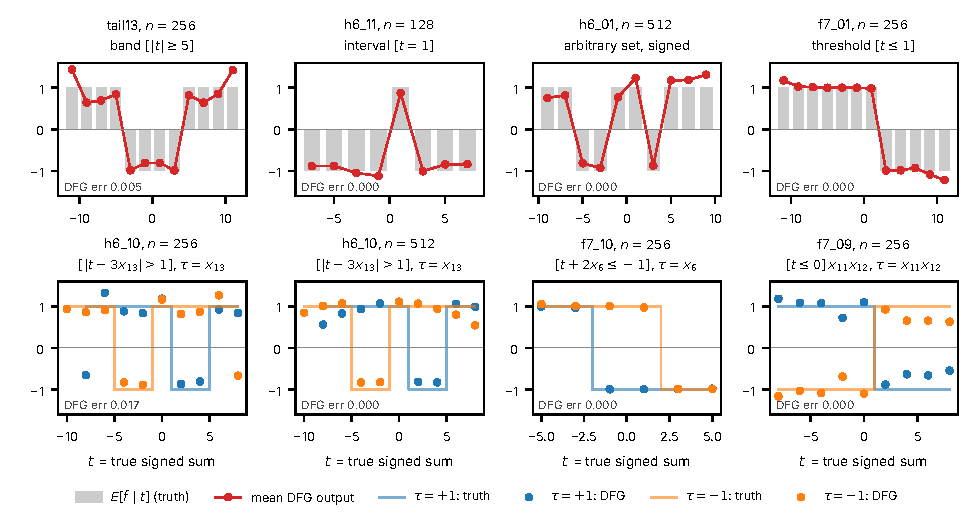
\includegraphics[width=\linewidth]{figures/fig_toy_g.pdf}
\caption{The learned function of the true block statistic $t$ (seed 0) \status{Numerical}. Top: grey bars are $E[f\mid t]$ over the 4096 test inputs; red points are the mean output of the whole DFG model at each level of $t$. Bottom: the same split by the second term $\tau$, from refits that reproduce the analysed cells. The plotted value is the conditional mean of the whole model, which includes spectral features, characters and stray product terms, not the block's own coefficients. Levels with fewer than 5 test points are not drawn; for h6\_10 at $n=256$ these include the cells $(t,x_{13})=(-10,+1)$ and $(10,-1)$, where the model is also wrong. ``DFG err'': the DFG member's test error. Source: the structure runs and \texttt{toy\_g} refits in \repo{study/part10/interp/results/toy_final/}.}
\label{fig:interp-toy-g}
\end{figure}

\paragraph{The learned function of the block} \status{Numerical} (\cref{fig:interp-toy-g}). Where the block is present, the model's mean output follows $E[f\mid t]$ level by level. This includes non-convex accept sets, such as h6\_01's $\{-9,-7,-5,-1,1,7,9\}$, and both branches of a weighted or modulated target. The values are not $\pm1$: the logistic readout rescales them and overshoots at rare extreme levels (tail13 at $|t|=11$). The panels add shape, not a new test. The share of test points at which the mean output has the sign of $E[f\mid t]$ is about one minus the DFG error by construction (0.983 for h6\_10 at $n=256$, 1.00 for the other seven panels). Below the discovery size the model has no block structure: for h6\_10 at $n=128$ the mean output is positive at every $(t,x_{13})$ level (0.01--0.90), so its sign agrees with $E[f\mid\cdot]$ only on the majority's 0.70 of the points, and the DFG error (0.39) is worse than a constant predictor's (0.30). The eight panels were chosen by hand; over all 53 exact cells of the 22 pure targets found, the agreement is at least 0.985 (\repo{study/part10/interp/VERIFICATION.json}, toy reading, C8).

\subsubsection{When the structure appears}\label{sec:interp-toy-timing}

\begin{figure}[tbp]
\centering
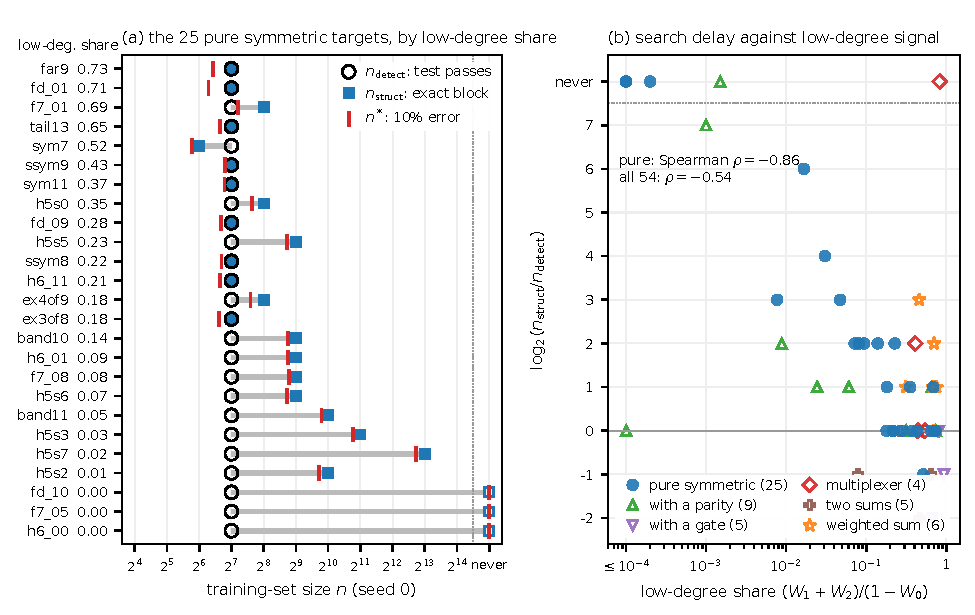
\includegraphics[width=\linewidth]{figures/fig_toy_timing.pdf}
\caption{When the structure appears (seed 0) \status{Numerical}. (a) The 25 pure symmetric targets, sorted by their share of variance at Fourier degrees 1--2 (number after the name). Open circle: $n_{\rm detect}$, the first grid size at which DFG's test would admit the true block. Square: $n_{\rm struct}$, the first grid size at which the model holds it exactly (open at ``never''); where $n_{\rm detect}=n_{\rm struct}$ the circle surrounds the square. Red tick: $n^*$, the 10\% test-error point of the same seed-0 fits, interpolated in $\log n$. The grey bar spans detection to discovery. (b) The delay $\log_2(n_{\rm struct}/n_{\rm detect})$ against the low-degree share for all 54 sum-structured targets; filled: pure symmetric, open: mixtures. Targets never found are drawn in the top row. Shares below $10^{-4}$ are drawn at $10^{-4}$, so h6\_00 and f7\_05 coincide at the top left. For the mixtures the detection points are the verifier's corrected ones (\cref{tab:interp-toy}). Spearman $\rho$ counts a target never found as $n_{\rm struct}=2^{15}$. No point is jittered. This figure replaces the analysis's \texttt{fig\_toy\_timing.pdf}, which used the uncorrected detection points. Sources: \repo{study/part10/interp/tables/toy_timing.csv} and \repo{study/part10/interp/VERIFICATION.json}.}
\label{fig:interp-toy-timing}
\end{figure}

\paragraph{Timing: the 25 pure symmetric targets} \status{Numerical}. On these targets the analysis is cleanest: the target is a function of one signed sum, and the round-0 test on the true block is close to the test DFG applies. \Cref{fig:interp-toy-timing}a shows each target.
\begin{itemize}
\item \emph{Detection is cheap.} The true block passes DFG's test at $n=128$ for all 25 targets. The test statistic grows linearly in $n$: its ratio to the threshold is at most 0.89 at $n=64$ and 1.07--1.78 at $n=128$.
\item \emph{Discovery is later where the low-degree signal is weak.} 22 of the 25 are found. Against $n_{\rm detect}$, $n_{\rm struct}$ is one doubling earlier for 1 target (sym7, held by the forced variant below the threshold), equal for 9, one doubling later for 3, and two or more later for 9 (band11, f7\_08, h6\_01, h5s2, h5s3, h5s5, h5s6, h5s7, band10).
\item \emph{The delay tracks the low-degree share} (\cref{fig:interp-toy-timing}b). Spearman's $\rho$ between the delay and $(W_1+W_2)/(1-W_0)$ is $-0.86$ over the 25 targets (a target never found counted as $n_{\rm struct}=2^{15}$), and $-0.80$ over the 22 found. The targets come from a few designed families, so a $p$-value that treats them as independent draws would overstate the evidence.
\item \emph{The readout is not the bottleneck.} For all 22 targets found, the seed-0 $n^*$ falls in the doubling just below $n_{\rm struct}$: the test error crosses 10\% between the last grid size without the exact block and the first with it. Because $n_{\rm struct}$ is a grid point and $n^*$ is interpolated, a finer statement cannot be made. In particular, the median offset of $\log_2(n^*/n_{\rm struct})$ ($-0.35$ over all 49 targets found) reflects the grid, not the readout.
\end{itemize}
\emph{Reading} \status{Heuristic}. For a function of one signed sum, DFG's data cost is set by its search, not by its test and not by its readout. Every seed of the block search reads the block's inputs off degree-1 and degree-2 statistics of the residual: prefixes of the top eigenvectors of the pair matrix, the degree-1 order and greedy growth from strong pairs (\cref{sec:dfg}). The weaker those statistics, the more data the search needs before it proposes the block, although the test would accept the block much earlier. No intervention isolates the search (such as seeding it with the true block); acceptance in later rounds and the stacker's choice of variant could also contribute.

\paragraph{The 29 mixtures} \status{Numerical}. For targets with a parity, gate, selector or second block, the round-0 test on the true block is a cruder proxy. With the verifier's corrected detection points (the modulated block tested on a residual already fitted on its modulator, as DFG tests it), 39 of the 54 targets are detectable at $n=128$, the median delay over the 49 found is 0 doublings, and Spearman's $\rho$ between delay and low-degree share over all 54 is $-0.54$ (\cref{app:interp-mixtures}).

\subsubsection{Where DFG fails: no low-degree foothold}\label{sec:interp-toy-fail}

\begin{figure}[tbp]
\centering
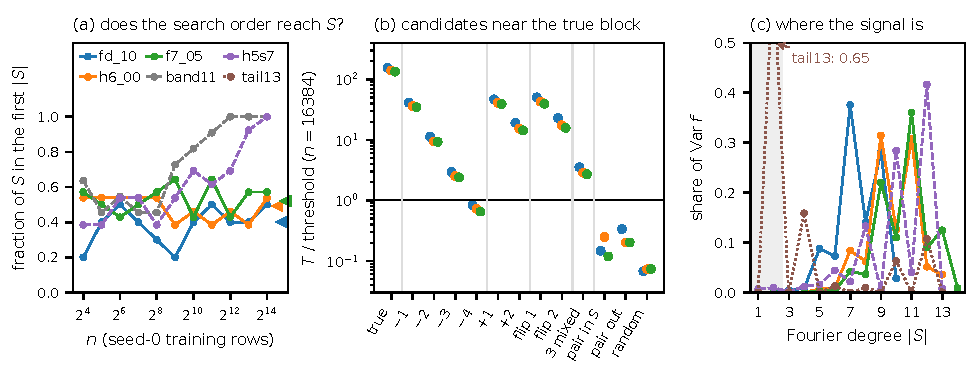
\includegraphics[width=\linewidth]{figures/fig_toy_failures.pdf}
\caption{Why the residue classes mod 3 are never found (seed-0 training rows) \status{Numerical}. (a) The fraction of the true class $S$ among the first $|S|$ inputs of the better of the search's two eigenvector orders. Triangles at the right edge: the value expected from the better of two random orders (0.40, 0.49, 0.52 for $|S|=10,13,14$). band11 and h5s7 are dashed (h5s7 also in (c)); they are found at the first $n$ at which all of $S$ lies within the order's first $|S|+5$ inputs (plotted fraction 0.82 and 0.92). The legend of (a) also serves (b) and (c). (b) DFG's test statistic over its threshold at $n=16384$ for the true block and for candidates near it: medians over 200 random candidates with 1--4 inputs dropped, 1--2 added, 1--2 signs flipped, or 3 errors of mixed kinds; the best 2-input block inside $S$; the best pair among 12 inputs outside $S$; random blocks of the true size. Above 1 the candidate passes. (c) The share of each target's variance by Fourier degree; degrees 1--2 shaded. tail13, found at $n=128$, has 0.65 at degree 2 (clipped). A compact version of the analysis's \texttt{fig\_toy\_failures.pdf}, with the chance level of panel (a) corrected for the better of two orders. Sources: \texttt{power/} and \texttt{toy\_landscape/} in \repo{study/part10/interp/results/toy_final/}.}
\label{fig:interp-toy-fail}
\end{figure}

\paragraph{The failures: residue classes mod 3} \status{Numerical}. Let $B=(s+k)/2$ count the $k$ signed inputs of the block that equal $+1$. Then fd\_10 $=[B\bmod3=0]$ on $k=10$ inputs, h6\_00 $=[B\bmod3\ne1]$ on 13 and f7\_05 $=[B\bmod3\ne0]$ on 14. Neither v3 nor v2 learns them (\cref{sec:res-toy-fail}). \Cref{fig:interp-toy-fail} shows why the search does not find them.
\begin{itemize}
\item \emph{The model.} At every $n\ge1024$ (fd\_10 from 128, f7\_05 from 256) the DFG model is the constant plus the kernel background. Its test error at $n=16384$ (0.32--0.34) is the test set's minority rate. For fd\_10 and h6\_00 these errors come from out-of-fold DFG fits on 13107 rows, which the stacker gave no weight. At smaller $n$ the forced variant adds 1--2 spurious characters or a spurious partial block (h6\_00 at $n=256$: $|-x_4+x_{12}-x_{22}-x_{23}|$, 2 of its 4 inputs in $S$).
\item \emph{The test would accept the block.} The true block passes from $n=128$ unfolded (512 folded). At $n=16384$ it is 155, 139 and 134 times the threshold.
\item \emph{There is no low-degree signal.} For h6\_00 and f7\_05, $W_1=W_2=0$ to five decimals; for fd\_10, $W_1=4\times10^{-5}$ and $W_2=1.7\times10^{-4}$. The Fourier weight peaks at degrees 7, 9 and 11.
\item \emph{The search's orders do not reach the block} (\cref{fig:interp-toy-fail}a). At $n=16384$ the eigenvector orders put 0.50, 0.54 and 0.57 of $S$ among their first $|S|$ inputs, against 0.40, 0.49 and 0.52 for the better of two random orders, and the fraction does not grow with $n$.
\item \emph{The basin is narrow} (\cref{fig:interp-toy-fail}b). At $n=16384$ the statistic falls about $4\times$ per missing input (to 41, 36 and 35 times the threshold with one input dropped; 2.9, 2.5 and 2.4 with three; 0.84, 0.73 and 0.65 with four). The first wrong sign or extra input costs $3.1$--$3.4\times$, the second $2.2$--$2.7\times$. Every sampled candidate with three errors of mixed kinds still passes. But no piece of the block carries signal: the best pair inside $S$ is at 0.15, 0.25 and 0.12 of the threshold, at the level of the best pair among 12 inputs outside $S$ (0.33, 0.20, 0.20), and random blocks of the true size are at 0.07. The basin estimate rests on medians of sampled candidates; other 4-error mixes were not measured.
\item \emph{A needle.} Within three errors of the true block there are $\sum_{j\le3}2^j\binom{30}{j}=34281$ candidates, against $\binom{30}{k}2^{k-1}=1.5\times10^{10}$, $4.9\times10^{11}$ and $1.2\times10^{12}$ blocks of the true size $k=10,13,14$.
\end{itemize}
\emph{Reading} \status{Heuristic}. A residue class mod 3 of a 10--14-input count is detectable once proposed and invisible from every low-order foothold the search has. For h6\_00 and f7\_05 the single and pair statistics are zero in expectation, so more data cannot help the seeds. For fd\_10 they are about 0.002, which the seeds could resolve only at $n$ of order $10^6$.

\paragraph{Late targets} \status{Numerical}. The pure targets found late, band11, h5s2, h5s3 and h5s7 (found at 1024--8192, with $W_1+W_2$ between 0.007 and 0.047), and h5s1, whose bottleneck is detecting its modulating parity, are consistent with the same mechanism in weaker form; h6\_08 and sumpar are late for representational reasons. Each is one seed (\cref{app:interp-late}).

% ==================================================================================================================
\subsection{Images: what the boosters split on}\label{sec:interp-img}

The analysis covers v3 on \code{qd_dev} at $n=1000$, 3000 and 10000, on \code{qd_a}, MNIST and Fashion-MNIST at $n=10000$, and v2 on \code{qd_dev} at $n=10000$. All four sets are development data for v3 (the held-out image sets are \code{qd_c} and \code{qd_d}), so the error comparisons below are in-sample; the held-out comparison is in \cref{sec:res-img-gain}. v2's analysis fit has test error 0.1467 against its multi-threaded evaluation cell's 0.1463 (\cref{sec:disc-provenance-disclosures}).
\begin{itemize}
\item \emph{Which booster is analysed.} The final \code{ggbt} and \code{cgbt} of each fit. On \code{qd_a} and MNIST the stacker gave \code{ggbt} weight 0, so it was not refitted, and the booster analysed is its out-of-fold fit on 8000 (7998) rows.
\item \emph{Geometry.} It is measured on the true $28\times28$ grid, which the learner never sees; for QuickDraw the columns are mapped back through the stored permutation. Distances are Chebyshev steps, so the 8 neighbours of a pixel are 1 step away.
\end{itemize}

\subsubsection{Pooling sets and bars on the true grid}\label{sec:interp-img-geom}

\begin{table}[tbp]
\centering{\footnotesize\setlength{\tabcolsep}{3.6pt}
\begin{tabular}{llrrrrrrrr}
\toprule
 & & \multicolumn{4}{c}{pooling sets: members other than $i$} & \multicolumn{2}{c}{Isomap $R^2$} & \multicolumn{2}{c}{bars: exact lines}\\
\cmidrule(lr){3-6}\cmidrule(lr){7-8}\cmidrule(lr){9-10}
set & $n$ & \hd{$S_i(4)$\\$\le1$ step} & \hd{$S_i(9)$\\$\le1$ step} & \hd{$S_i(9)$\\$\le2$ steps} & \hd{$S_i(9)$\\$>2$ steps} & \hd{$k=4$\\union} & \hd{$k=9$\\mutual} & $L=2$ & $L=4$\\
\midrule
\code{qd_dev} & 1000 & 0.983 & 0.823 & 0.985 & 79 & 0.84 & 0.87 & 0.33 & 0.16\\
\code{qd_dev} & 3000 & 0.991 & 0.829 & 0.991 & 46 & 0.97 & 0.89 & 0.38 & 0.21\\
\code{qd_dev} & 10000 & 0.994 & 0.834 & 0.994 & 31 & 0.97 & 0.92 & 0.42 & 0.24\\
\code{qd_a} & 10000 & 0.999 & 0.817 & 0.989 & 59 & 0.99 & 0.83 & 0.40 & 0.25\\
MNIST & 10000 & 0.976 & 0.787 & 0.966 & 186 & 0.92 & 0.97 & 0.20 & 0.06\\
Fashion & 10000 & 0.881 & 0.633 & 0.840 & 1006 & 0.13 & 0.23 & 0.11 & 0.04\\
\bottomrule
\end{tabular}
}
\caption{The pooling sets and bars of v3's image members on the true pixel grid (seed 0) \status{Numerical}. Pooling sets: the fraction of the $k-1$ members of $S_i(k)$ other than $i$ itself that lie within 1 or 2 Chebyshev steps of $i$, over all non-constant pixels $i$; ``$>2$ steps'': the number of such members (of 5408 on QuickDraw at $k=9$). Isomap $R^2$: Procrustes $R^2$ between a 2-D Isomap embedding of the pooling-set graph (an edge from $i$ to each member of $S_i(k)$; ``mutual'': only edges in both directions) and the true pixel coordinates. Bars: the fraction of bars of half-length $L$ whose pixels lie on one horizontal, vertical or diagonal lattice line. MNIST's $k=9$ mutual graph covers 674 of its 682 non-constant pixels. Source: the analysis files in \repo{study/part10/interp/results/image_final/v3/}.}
\label{tab:interp-img-geom}
\end{table}

\paragraph{Pooling sets are local neighbourhoods; on Fashion-MNIST some include the mirror pixel} \status{Numerical}. \Cref{tab:interp-img-geom} gives the geometry.
\begin{itemize}
\item \emph{QuickDraw.} 98.3--99.9\% of the other members of $S_i(4)$ lie within one step of $i$, and 98.5--99.4\% of those of $S_i(9)$ within two. Only 8 pixels lie within one step, so for $k=16$ at most $8/15=0.53$ of the other members can; 0.49 do. On \code{qd_dev} the members of $S_i(9)$ farther than two steps fall from 79 to 31 as $n$ grows from 1000 to 10000. The sets overlap the $k$ truly nearest pixels by 0.82, 0.88 and 0.78 for $k=4$, 9 and 16 at $n=10000$.
\item \emph{MNIST.} The 23 far members of $S_i(4)$ sit at 13 border pixels that are nonzero in at most 0.04\% of the 10000 training images. Their correlations rest on a handful of images.
\item \emph{Fashion-MNIST.} At 57 of the 784 pixels (7\%), $S_i(4)$ contains a far member, and all 65 far members are the centre's mirror pixel: the same row $\pm1$, with columns summing to $27\pm2$. At $k=9$, 619 of the 1006 far members are mirror pixels.
\end{itemize}
\emph{Reading} \status{Heuristic}. Garments are nearly left--right symmetric, so a pixel can correlate with its mirror image as strongly as with its neighbours. Sets at those pixels pool both sides of the garment.

\paragraph{The grid is recovered globally on QuickDraw and MNIST} \status{Numerical}. The 2-D Isomap embedding \cite{tenenbaum2000global} of the $k=4$ pooling-set graph matches the true grid with Procrustes $R^2$ 0.97--0.99 on QuickDraw at $n\ge3000$ (0.84 at $n=1000$), 0.92 on MNIST and 0.13 on Fashion-MNIST. Variants of the graph with a few long edges score much lower (\cref{app:interp-img-more}). The learner never builds a global embedding; it uses each set as a local sum. So $R^2$ summarizes how map-like the recovered neighbourhoods are, not a property the learner uses.

\begin{figure}[tbp]
\centering
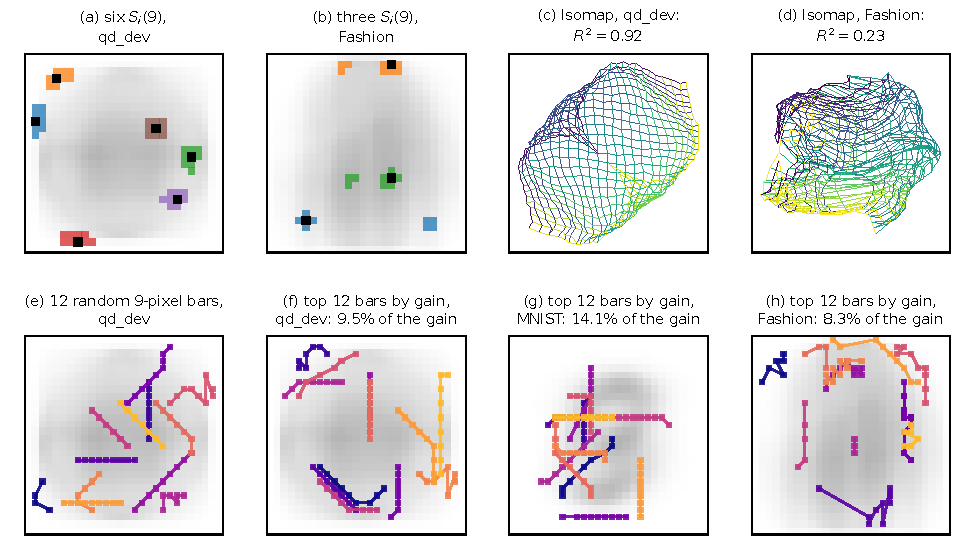
\includegraphics[width=\linewidth]{figures/fig_img_grid.pdf}
\caption{Pooling sets and bars of v3 on the true pixel grid, $n=10000$, seed 0 \status{Numerical}. Background: the average of the ten class-mean training images. (a) $S_i(9)$ at six pixels of \code{qd_dev} (black: $i$). (b) $S_i(9)$ at three inked Fashion-MNIST pixels whose sets contain mirror pixels. (c, d) The 2-D Isomap embedding of the $k=9$ mutual pooling-set graph, Procrustes-aligned to the grid and drawn as the true lattice: each pixel at its embedded position, joined to its horizontal and vertical grid neighbours (horizontal edges coloured by row, vertical edges by column). (e) Twelve randomly chosen 9-pixel bars ($L=4$) of \code{qd_dev}. (f--h) The twelve 9-pixel bars with the most split gain in \code{cgbt}, with their combined share of \code{cgbt}'s total gain. In (e)--(h) colour only distinguishes bars (in (f)--(h) darker means more gain); a bar's pixels are joined in order along its principal axis, so a long segment joins two separate pieces of one bar. Simplified from \texttt{fig\_img\_topology.pdf} and \texttt{fig\_img\_bars.pdf} in \repo{study/part10/interp/figures/}.}
\label{fig:interp-img-grid}
\end{figure}

\paragraph{Bars are short, nearly straight runs along recovered lines} \status{Numerical} (\cref{tab:interp-img-geom}, \cref{fig:interp-img-grid}).
\begin{itemize}
\item \emph{Shape on \code{qd_dev}.} At $n=10000$, 42\% of the 5-pixel bars ($L=2$) are exact lattice lines, and 96\% stay within one pixel of their principal axis. For the 9-pixel bars ($L=4$) the figures are 24\% and 63\%, since each further step can turn.
\item \emph{Growth with $n$.} The exact-line fraction grows with $n$ (0.33, 0.38, 0.42 for $L=2$ at $n=1000$, 3000, 10000; 0.16, 0.21, 0.24 for $L=4$). The within-one-pixel fraction does not, and it is a weak criterion for 5 pixels.
\item \emph{Orientation.} On QuickDraw all four orientations occur about equally often; on Fashion-MNIST horizontal and vertical bars dominate (0.37 and 0.40 at $L=2$).
\item \emph{Other sets.} On MNIST the bars are less straight (0.20 and 0.06 exact lines). On Fashion-MNIST they are rarely lines (0.11 and 0.04), and 27\% ($L=2$) and 30\% ($L=4$) contain a mirror pixel, against 2\% and 9\% on \code{qd_dev}. There a bar is often two short pieces on the two sides of the garment (\cref{fig:interp-img-grid}h).
\end{itemize}
Straightness is a property of the construction and the data, not of anything the booster learned.

\subsubsection{Which members carry v3}\label{sec:interp-img-members}

\begin{table}[tbp]
\centering{\footnotesize\setlength{\tabcolsep}{3.2pt}
\begin{tabular}{llrrrrrrrrrrr}
\toprule
 & & \multicolumn{6}{c}{share of the stacking weight} & \multicolumn{2}{c}{\hd{out-of-fold\\error}} & \multicolumn{3}{c}{test error}\\
\cmidrule(lr){3-8}\cmidrule(lr){9-10}\cmidrule(lr){11-13}
set & $n$ & \code{cgbt} & \code{ggbt} & \code{gknn} & \code{knn} & \hd{\code{gbt},\\\code{et}} & \code{lin_C} & \code{cgbt} & \code{ggbt} & stack & \hd{\code{cgbt}\\alone} & \hd{\code{ggbt}\\alone}\\
\midrule
\code{qd_dev} & 1000 & 0.32 & 0.09 & 0.44 & 0.16 & 0.00 & 0.00 & 0.272 & 0.280 & 0.2118 & 0.2208 & 0.2478\\
\code{qd_dev} & 3000 & 0.40 & 0.08 & 0.33 & 0.19 & 0.00 & 0.00 & 0.197 & 0.212 & 0.1753 & 0.1851 & 0.1968\\
\code{qd_dev} & 10000 & 0.47 & 0.07 & 0.17 & 0.25 & 0.03 & 0.00 & 0.149 & 0.161 & 0.1330 & 0.1368 & 0.1578\\
\code{qd_a} & 10000 & 0.56 & 0.00 & 0.15 & 0.24 & 0.06 & 0.00 & 0.161 & 0.172 & 0.1422 & 0.1442 & 0.1654$^a$\\
MNIST & 10000 & 0.40 & 0.00 & 0.23 & 0.24 & 0.13 & 0.00 & 0.031 & 0.043 & 0.0255 & 0.0278 & 0.0392$^a$\\
Fashion & 10000 & 0.10 & 0.16 & 0.00 & 0.04 & 0.50 & 0.20 & 0.126 & 0.127 & 0.1238 & 0.1216 & 0.1222\\
\addlinespace
v2, \code{qd_dev} & 10000 & -- & 0.41 & 0.24 & 0.24 & 0.11 & 0.00 & -- & 0.161 & 0.1467 & -- & --\\
\bottomrule
\end{tabular}
}
\caption{Which members carry v3 on images (seed 0, one fit each) \status{Numerical}. Left: each member family's share of the total stacking weight. \code{gknn}: $k$-NN votes on pooled sums; \code{knn}: $k$-NN votes on pixels; \code{gbt}, \code{et}, \code{lin_C}: Part 8's LightGBM, ExtraTrees and logistic regression on pixels. Middle: out-of-fold error of the two boosters (5-fold at $n\le3000$; one holdout of 2000 rows at $n=10000$). Right: test error of the stacked learner (v3; v2 in the last row) and of each booster alone (its own argmax). $^a$\code{ggbt} had stacking weight 0, so the booster shown is its out-of-fold fit on 8000 (\code{qd_a}) or 7998 (MNIST) rows; only the out-of-fold comparison is like for like there. Last row: v2's analysis fit. The weights are not shares of the decision (see the cautions in the text). Source: the analysis files in \repo{study/part10/interp/results/image_final/}.}
\label{tab:interp-img-stack}
\end{table}

\paragraph{\code{cgbt} is the member that carries v3 on QuickDraw and MNIST} \status{Numerical} (\cref{tab:interp-img-stack}).
\begin{itemize}
\item \emph{The best member.} \code{cgbt} has the lowest out-of-fold error of all 18 members in every v3 fit. The margin over \code{ggbt} is within holdout noise on Fashion-MNIST and at \code{qd_dev}, $n=1000$. It has the largest single-member weight everywhere except Fashion-MNIST, where Part 8's \code{gbt} has it.
\item \emph{Its weight.} Its share of the stacking weight grows with $n$ on \code{qd_dev} (0.32, 0.40, 0.47) and is 0.56 on \code{qd_a}, 0.40 on MNIST and 0.10 on Fashion-MNIST.
\item \emph{\code{ggbt} loses its weight.} At \code{qd_dev}, $n=10000$, \code{ggbt}'s share falls from 0.41 in v2's fit (0.37 in v2's evaluation cell) to 0.07 in v3. On \code{qd_a} and MNIST it is 0.
\item \emph{The rest of the weight.} Most of it goes to the $k$-NN members, on pooled sums and on pixels. On Fashion-MNIST half goes to Part 8's \code{gbt} and \code{et} and a fifth to logistic regression.
\item \emph{Alone.} On the test set \code{cgbt} alone beats \code{ggbt} alone on QuickDraw and MNIST (on \code{qd_a} and MNIST against \code{ggbt}'s out-of-fold fit on fewer rows; the like-for-like out-of-fold errors, 0.161 against 0.172 and 0.031 against 0.043, point the same way): 13.68\% against 15.78\% at \code{qd_dev}, $n=10000$. The two agree on 89--98\% of test points. The stack is 0.2--1.0 points better than \code{cgbt} alone on QuickDraw and MNIST; the 0.2 points on \code{qd_a} are not resolved by the test set. On Fashion-MNIST the stack (12.38\%) is not better than either booster alone (12.16\%, 12.22\%), a difference the test set does not resolve either.
\end{itemize}
Three cautions apply to the stacking weights, here and in \cref{tab:img-stack}.
\begin{itemize}
\item They act on log-probabilities of different calibration. Boosters stopped early on error give over-confident log-probabilities (clipped at $10^{-5}$), while $k$-NN votes, ExtraTrees and logistic regression are smoother. Equal weights are not equal influence.
\item The convex stacker splits weight between two nearly collinear boosters on one 2000-row holdout, so ``\code{ggbt} gets weight 0'' describes one fit. The 8 held-out fits at $n\ge10000$ show the same shift (\cref{sec:res-img-gain}).
\item The out-of-fold errors at $n=10000$ rest on those 2000 rows. Unpaired, the standard error of an error near 0.15 is about 0.008; for two members on the same rows the paired one is smaller.
\end{itemize}

\begin{table}[tbp]
\centering{\footnotesize\setlength{\tabcolsep}{4pt}
\begin{tabular}{lrrrrrr}
\toprule
 & \multicolumn{4}{c}{\code{cgbt}} & \multicolumn{2}{c}{\code{ggbt}}\\
\cmidrule(lr){2-5}\cmidrule(lr){6-7}
feature type & \code{qd_dev} & \code{qd_a} & MNIST & Fashion & \code{qd_dev} & Fashion\\
\midrule
pixels & 0.01 (0.1) & 0.01 (0.1) & 0.01 (0.1) & 0.09 (1.0) & 0.04 (0.1) & 0.16 (0.7)\\
pooled sums, $k=4$ & 0.02 (0.3) & 0.03 (0.3) & 0.05 (0.6) & 0.10 (1.1) & 0.10 (0.4) & 0.15 (0.7)\\
pooled sums, $k=9$ & 0.04 (0.5) & 0.05 (0.5) & 0.07 (0.9) & 0.10 (1.2) & 0.16 (0.7) & 0.16 (0.7)\\
pooled sums, $k=16$ & 0.15 (1.8) & 0.12 (1.5) & 0.07 (0.8) & 0.12 (1.4) & 0.32 (1.5) & 0.15 (0.6)\\
bars, $L=2$ & 0.24 (0.7) & 0.25 (0.8) & 0.30 (0.9) & 0.25 (0.7) & -- & --\\
bars, $L=4$ & 0.53 (1.6) & 0.54 (1.6) & 0.51 (1.5) & 0.35 (1.1) & -- & --\\
prototype pairs & -- & -- & -- & -- & 0.39 (4.1) & 0.38 (4.4)\\
\addlinespace
all bars & 0.77 (1.2) & 0.79 (1.2) & 0.80 (1.2) & 0.60 (0.9) & -- & --\\
all pooled sums & 0.22 (0.9) & 0.20 (0.8) & 0.19 (0.8) & 0.31 (1.3) & 0.57 (0.9) & 0.46 (0.7)\\
\midrule
columns & 8220 & 8220 & 8286 & 9408 & 3112 & 3436\\
\bottomrule
\end{tabular}
}
\caption{Split gain by feature type in the final boosters, $n=10000$, seed 0 \status{Numerical}. Each entry is the type's share of the booster's total split gain, with its ratio to the type's share of the columns in brackets (1.0: as much gain per column as the booster's average). Bars are two thirds of \code{cgbt}'s columns; the 300 prototype pairs are about a tenth of \code{ggbt}'s. LightGBM samples 5\% (\code{cgbt}) or 12\% (\code{ggbt}) of the columns per tree. \code{ggbt} on \code{qd_a} and MNIST, an out-of-fold fit, is not shown (pairs 0.30 and 0.41 of its gain). Split gain describes how the trees split, not what the predictions depend on. Source: the analysis files in \repo{study/part10/interp/results/image_final/v3/}.}
\label{tab:interp-img-gain}
\end{table}

\paragraph{Split gain by feature type} \status{Numerical} (\cref{tab:interp-img-gain}).
\begin{itemize}
\item \emph{The bars in \code{cgbt}.} The bars carry 0.77--0.80 of \code{cgbt}'s split gain on QuickDraw and MNIST at $n=10000$ (0.72 at \code{qd_dev}, $n=1000$) and 0.60 on Fashion-MNIST. They are two thirds of its columns, so this is 1.1--1.2 times their column share (0.9 on Fashion-MNIST): more than their share, not dominance. They also make 0.75 of the splits at \code{qd_dev}, $n=10000$. Per column, the 9-pixel bars (1.5--1.6; 1.1 on Fashion-MNIST) and, on QuickDraw, the 16-pixel pooled sums (1.5--1.8) carry the most. The 5-pixel bars carry 0.7--0.9 of the average, and single pixels 0.1, except on Fashion-MNIST (1.0).
\item \emph{The pairs in \code{ggbt}.} The 300 prototype pairs carry about 0.4 of \code{ggbt}'s gain (0.30 in \code{qd_a}'s out-of-fold fit), about four times their column share. On \code{qd_dev} the 16-pixel pooled sums come next (1.5).
\item \emph{Use is wide, gain concentrated.} Almost every bar is split on at least once (at \code{qd_dev}, $n=10000$: 2520 and 2596 of 2704 for $L=2$ and 4). But the top 10\% of bars carry 0.65--0.66 of the bar gain there (0.76 at $n=1000$), 0.78--0.84 on Fashion-MNIST and 0.86 on MNIST. The twelve 9-pixel bars with the most gain carry 9.5\%, 14.1\% and 8.3\% of \code{cgbt}'s total gain on \code{qd_dev}, MNIST and Fashion-MNIST (\cref{fig:interp-img-grid}f--h).
\end{itemize}

\paragraph{v3 against v2 at \code{qd_dev}, $n=10000$} \status{Numerical}. The two fits have identical pooling sets and a bit-identical \code{ggbt}: the same gain vector, test predictions and maps, and 123 rounds in both. So, as far as checked, the fits differ by \code{cgbt}, the stacking weights, and which members are refitted. The errors are 0.1467 for v2 and 0.1330 for v3. 2.08\% of the test points are right in v3 and wrong in v2, and 0.71\% the reverse. Per-class detail is in \cref{app:interp-v2}.

\subsubsection{Class evidence maps}\label{sec:interp-img-maps}

\paragraph{Class evidence maps: method and limits.} For each class, 100 test points of that class are taken. LightGBM's TreeSHAP contributions \cite{lundberg2020local} of each feature to that class's raw score are computed and spread over pixels. A pixel keeps its own contribution. A pooled sum or bar spreads its contribution equally over its pixels. A prototype pair $u=x_a-x_b$ spreads it over pixels $j$ in proportion to $|u_jx_j|$. The maps are averaged over the 100 points. They can show where in the image the features that raise a class's score look. They cannot show more than that, for five reasons.
\begin{itemize}
\item \emph{Own score only.} A map is the contribution to the class's own raw score in a 10-class softmax, not to its margin over the other classes.
\item \emph{No causal test.} Nothing was occluded or ablated, so no region is shown to be necessary.
\item \emph{The spreading rule.} Spreading a subset sum equally over its pixels books part of the evidence of a partly inked bar on blank pixels. On \code{qd_dev}, of the members of bars with at least one inked member, 43\% ($L=2$) and 52\% ($L=4$) are blank. So evidence on blank pixels marks where a feature looks, not necessarily what drove it.
\item \emph{Built-in agreement.} The pairs' maps follow the class's own ink by construction. \code{cgbt} and \code{ggbt} share the pixels, the pooled sums and the spreading rule, so part of their agreement is built in.
\item \emph{Post-hoc regions.} The regions named in the Reading and in \cref{app:interp-maps-ex} were drawn after looking at the maps. Their shares describe the maps; they do not test them.
\end{itemize}

\begin{figure}[tbp]
\centering
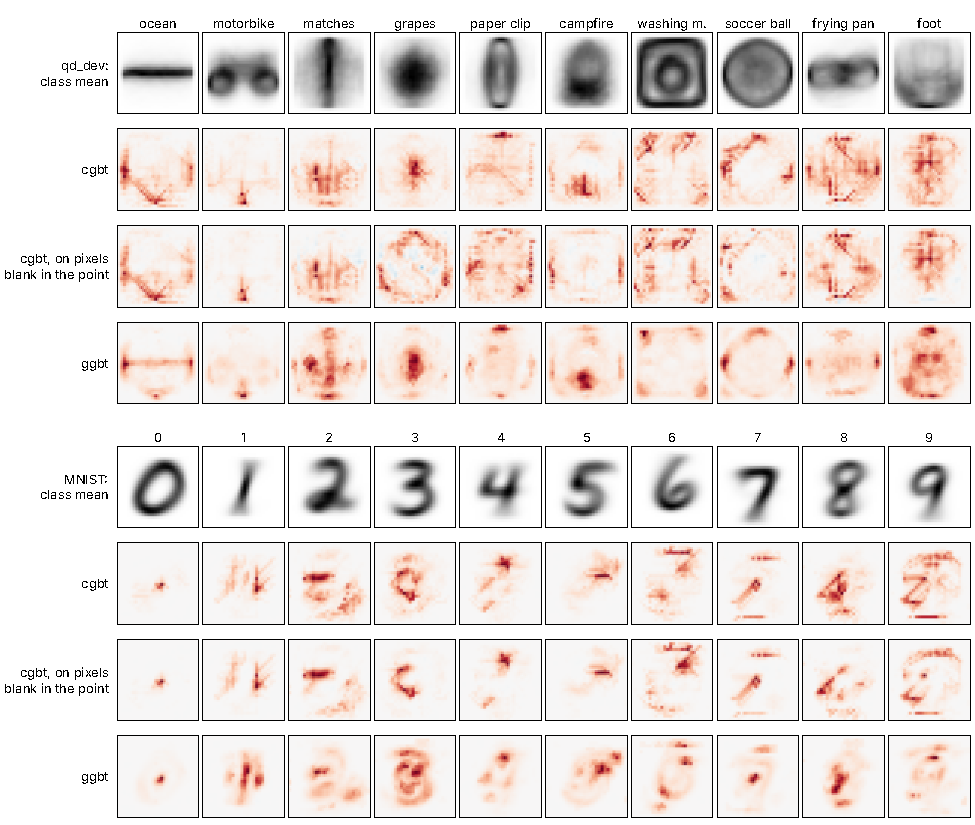
\includegraphics[width=\linewidth]{figures/fig_img_contrib.pdf}
\caption{Class evidence maps of v3's two boosters on \code{qd_dev} and MNIST, $n=10000$, seed 0 \status{Numerical}. Each map is the mean, over 100 test points of the class, of the TreeSHAP contributions to that class's own raw score, spread over pixels as described in the text; red is positive, and each map is scaled to its own 99th percentile of $|$value$|$ (the top 1\% saturate). Rows: the class's mean training image; \code{cgbt}; the part of \code{cgbt}'s map on pixels blank in the point ($x\le0.1$); \code{ggbt}, prototype pairs included. The maps are descriptive (see the text for what they cannot show). Simplified from \texttt{fig\_img\_contrib\_qd\_dev.pdf} and \texttt{fig\_img\_contrib\_mnist.pdf} in \repo{study/part10/interp/figures/}, which also show the pooled-sum and pair parts, and Fashion-MNIST and \code{qd_a}.}
\label{fig:interp-img-contrib}
\end{figure}

\paragraph{What the maps show} \status{Numerical} for the shares (\cref{fig:interp-img-contrib}).
\begin{itemize}
\item \emph{Sign.} The mean maps are almost all positive: positive values make at least 0.96 of each map's absolute mass.
\item \emph{Blank pixels.} The share of the net evidence on pixels blank in the point, averaged over classes, is 0.61 for \code{cgbt} on \code{qd_dev}, 0.56 on Fashion-MNIST, 0.69 on MNIST and 0.62 on \code{qd_a}. For \code{ggbt} it is 0.39--0.44, and 0.53--0.68 once its pairs are removed. Blank pixels are 0.75, 0.73, 0.83 and 0.55 of these images (\code{qd_dev}, \code{qd_a}, MNIST, Fashion-MNIST), so per pixel, inked pixels carry more of the evidence on QuickDraw and MNIST, and Fashion-MNIST is at par. It is not so for every class: grapes, soccer ball and campfire (0.32--0.39 on \code{qd_dev}), pullover, shirt and coat (0.25--0.29), camouflage on \code{qd_a} (0.15) and the digit 8 (0.42) draw most of their evidence from ink.
\item \emph{Agreement.} The \code{cgbt} and \code{ggbt} maps of a class correlate at 0.63--0.94 on \code{qd_dev}, Fashion-MNIST and MNIST, and at 0.40--0.88 on \code{qd_a} (slightly less over non-constant pixels only: 0.60--0.94 and 0.33--0.87).
\item \emph{By feature type.} By absolute contribution, \code{cgbt}'s evidence on \code{qd_dev} is 0.78 bars, 0.20 pooled sums and 0.02 pixels. \code{ggbt}'s is 0.64 pooled sums, 0.29 pairs and 0.07 pixels.
\end{itemize}
\emph{Reading} \status{Heuristic}. In these maps a sizable part of a class's evidence sits where the class has no ink and other classes do; for several digits the largest named region is an open one (0, 1, 3, 4, 7). Two examples (shares \code{cgbt} / \code{ggbt} of the class's net evidence): on MNIST the hole of the 0 carries 0.46 / 0.41 of the evidence on 3\% of the image, 99\% of it on blank pixels; on \code{qd_dev} the blank gap between a motorbike's wheels carries 0.20 / 0.16 (\cref{app:interp-maps-ex} lists the others). \code{cgbt} does not look at different places from \code{ggbt}. It looks at the same places through thinner, oriented windows: lines and chains of short segments, where \code{ggbt}'s pooled sums give blobs. That difference in shape follows from the feature shapes and is not learned. What the fit chose is which segments carry weight.

\section{Discussion}\label{sec:discussion}

\subsection{What kind of learner this turned out to be}\label{sec:disc-kind}

v3 is not one mechanism but three learners under one convex stacker, and the input type decides which of them carries the fit (\cref{sec:learner}): enumerate-and-test on Boolean inputs, at about an Occam sample cost wherever its search can propose the right feature \status{Heuristic}; a fixed, data-derived hierarchy of subset sums read out by gradient-boosted trees on images, with nothing fitted inside the features; and the classical stack of Part 8 on other tabular data. That is the AutoML-style dispatch by input type of the Parts 6--9 paper (\cref{sec:relates}), and Part 10's two additions, a wider sum-block search for DFG and a second booster over a richer bank, sit inside the first two regimes. What the results add is where each regime's performance comes from. On Boolean inputs, the interpretability analysis places DFG's data cost in its search's low-degree seeds rather than in its test (\cref{sec:interp-toy}; a reading of descriptive measurements, not an ablation). On images, the gain over v2 is a better fixed representation, which ties a CPU-matched MLP ensemble at $n=60000$ (\cref{sec:res-img-gain}). On tabular data nothing has changed since Part 8 (\cref{sec:res-tabular}).

\subsection{Why it works where it works}\label{sec:disc-why}

\paragraph{Boolean targets: an Occam-like sample cost, when the search can propose} \status{Heuristic}. DFG's test admits a feature once $n$ exceeds a multiple of the log-size of its class over the squared residual correlation (\cref{sec:dfg}). For a $k$-sparse character, $\ln N\approx k\ln d$; for a signed block on $k$ of $d$ inputs, $\ln N\approx\ln\bigl(\binom dk2^{k-1}\bigr)$. Either way the sample cost is logarithmic in the size of the dictionary: the Occam rate, paid for with FLOPs of enumeration and search that fit inside one network run at $d=30$. Gradient-trained networks pay in samples instead. For parities the companion paper measured rates close to the leap and correlational-SQ rate $d^{k-1}$ \cite{gdcircuit2026,abbe2022msp,abbe2023leap,barak2022hidden,kearns1998sq}. For an even function of one signed sum, a network has to find the block's sign vector in the degree-2 statistic $\E[f\,xx^\top]$ against sampling noise. That is the information-exponent picture of single-index learning \cite{benarous2021online,damian2024gaps}. Networks can trade data for width and compute along a frontier \cite{edelman2023pareto}; DFG sits at an extreme of that trade.

The interpretability analysis sharpens the picture in one respect (\cref{sec:interp-toy}). On the pure symmetric targets the test is not the bottleneck, and the data cost is consistent with being set by when the search first \emph{proposes} the block, which it seeds from degree-1 and degree-2 statistics of the residual (findings 2 and 3 of \cref{sec:interp}). So DFG relies on the same low-order statistics that a network's gradient sees. It needs far fewer samples because it rounds a coarse spectral estimate to an exact signed subset and then tests that subset with a union bound, where a network has to learn the direction to useful precision by noisy local steps \status{Heuristic}.

\paragraph{Where neither has a foothold.} The residue classes mod 3 of 10--14-input counts have almost no Fourier weight at degrees 1 and 2, and DFG's search never proposes their block, although the test would accept it long before $n=16384$ (\cref{sec:interp-toy-fail}). The networks mostly fail too: none learns f7\_05, and only the most regularized variant learns h6\_00, at $\nstar=12304$ (fd\_10, in \code{dlfamdev}, has no network runs). Their signal sits at high degree on an unknown subset of inputs, which learners that rely on low-order correlations should find hard \cite{kearns1998sq}. Exhaustive search does not help within the budget: there are $1.5\times10^{10}$ to $1.2\times10^{12}$ blocks of the true size, each costing at least $n$ operations to score, against $1.62\times10^{11}$ FLOPs per toy fit. So this is a shared limit, not a loss specific to discrete search \status{Heuristic}. The only target on which a network is clearly better than v3 is of this kind.

\paragraph{Images: locality recovered from data, read out by trees} \status{Heuristic}. On QuickDraw the most correlated pixels of a pixel are its neighbours, so the pooling sets are small blobs of the true grid and the bars short runs along it (\cref{sec:interp-img-geom}). Recovering image topology from such correlations is an old idea \cite{leroux2007topology}, as is grouping inputs into receptive fields by correlation \cite{coates2011receptive}. Boosted trees \cite{ke2017lightgbm} over these fixed local sums then do what a first convolutional layer with a nonlinearity would do, but at fixed positions and without shared weights. The MLP references are denied this structure by design: they are invariant to the pixel permutation, and nothing in their training recovers it. So v3 beats MLP ensembles that spend 2.0 and 5.0 times its FLOP budget (\code{mlp_strong} at all six held-out cells, \code{mlp_wide} at five of six), and ties the 1024-wide ensemble, which spends 9.2 budgets and a comparable time per fit. The control and context runs bound how much of this is representation (\cref{sec:res-img-gain}): an MLP given v2's pooled sums ties v2 but not v3, no MLP was given the bars, and a CNN told the layout (seed 0) has lower error at all three cells where both ran, clearly at one. It does not show that discrete search beats gradient-based learning on images.

\paragraph{Tabular data} \status{Heuristic}. Here the result is the known strength of tree ensembles and stacking on medium-sized tabular data against standard-recipe MLPs (\cref{sec:res-tabular}); DFG runs on 2 of the 26 datasets and changes no cell there clearly.

\subsection{Limits}\label{sec:disc-limits}

\begin{itemize}
\item \textbf{Small held-out sets.} \code{dlheld7} has 12 targets from one family, and on 5 of its 10 wins default gradient boosting or logistic regression already beats the networks. \code{qd_c} and \code{qd_d} are two 10-class sets from one source. The 10 fresh tabular datasets of Part 8 give $p=0.11$. A second family or source could change the picture.
\item \textbf{The earlier suites are in-sample} (\cref{sec:discipline}). Pooled numbers over all suites summarize the record; they are not held-out estimates. The margin against \code{nets_wd} is smallest on the two draws of the blind family, which is what selection on the other suites would produce, though the suites also differ in kind and the differences are within noise (\cref{sec:res-toy-all}).
\item \textbf{One seed at $n\ge30000$ on images.} The two cells that decide the comparison with \code{mlp_xl} rest on one fit each, and on the test set's binomial noise for their standard error. v3's gain over v2 is below the 10\% threshold at every held-out cell; that v3 is lower in all 14 seed-paired fits is a description, not a pre-registered test (\cref{sec:res-img-heldout}).
\item \textbf{Targets without a low-degree foothold} are found late or never: the residue classes mod 3 never, h5s7 at $n=8192$, and h5s1 in no learner's 3-seed mean (\cref{sec:res-toy-fail,sec:interp-toy-fail}). No cheap search for them is known (\cref{sec:disc-next}).
\item \textbf{Locality is used in spirit.} The image members never read a pixel index, but the correlations give back neighbourhoods and lines, the information the permuted-pixel protocol was meant to withhold (\cref{sec:interp-img-geom}). No MLP was given the bars, and a CNN told the layout has lower error wherever both ran (\cref{sec:res-img-gain}).
\item \textbf{Equal FLOPs are not equal CPU time, and prediction is not charged.} v3 uses 0.30--0.58 of its FLOP budget on the held-out cells, but takes about as long per fit as \code{mlp_xl}, which it only ties. At $n=3000$ it is close to the budget guard once Part 9's audited correction is applied, and no compute audit of v3 was made. A v2 query costs about $500\times$ an MLP's, and v3 adds to it (\cref{sec:res-img-compute}).
\item \textbf{Concrete references.} One toy network architecture at one width and one learning rate, and image MLPs without augmentation or architecture search. The hindsight minima favour the references, but stronger networks would plausibly narrow the margins.
\item \textbf{No independent audit in Part 10.} Parts 8 and 9 had independent audits of leakage, compute, discreteness and reference strength \cite{discretelearners2026}. Part 10 inherits their findings and fixes, but its own comparisons were not re-audited in that sense. The interpretability analyses were independently verified, and the paper's claims were checked against the result files and records by independent checkers (\cref{app:provenance}).
\item \textbf{The interpretability is descriptive}: seed 0, no ablation of the learner or causal test, mechanism labels for v1.3's changes read off fitted models, and stacking weights, split gain and contribution maps that describe the fits, not what their predictions depend on (\cref{sec:interp}).
\end{itemize}

\subsection{What would test it further}\label{sec:disc-next}

\begin{enumerate}
\item \emph{The information-matched image comparison.} Give an MLP v3's whole bank, pooled sums and bars, as \code{mlp_pool} did for v2's. Train a gradient-based network that learns sparse local connectivity \cite{neyshabur2020convolutions}, or a locally connected network on the recovered neighbourhoods. Either would say how much of v3's image margin is representation that a network can use as well.
\item \emph{A second blind toy family}, written independently of the first, and the toy suites at larger $d$. At $d=30$ the advantage on the blind family is a factor of about $2^{1.5}\approx2.8$. For parities DFG's advantage grew with $d$ in Part 6; whether it does for signed sums was not measured.
\item \emph{Block search beyond degree 2.} A seed that reads higher-order statistics of the residual could reach the mod-$q$ targets. The Part 10 builder found that the true block of fd\_10 is detectable only within about 3--4 errors of the truth, so that random restarts would need far more than $10^5$ tries; a cheaper route is not known.
\item \emph{Power and attribution.} More seeds at $n=60000$; a pre-registered paired comparison with v2; image sets from another source; ablations of v1.3's three additions on held-out targets; and a compute audit of v3 that also charges prediction.
\end{enumerate}


\bibliographystyle{plainnat}
\bibliography{refs}

\appendix
\section{How Part 10 was run}\label{app:provenance}

Part 10 and this paper were produced by an AI system, Claude (Anthropic), on 27--28 October 2026. Kaarel H\"anni posed the request: ``a couple more hours'' on a better discrete learner, then interpretability of the best learner so far, and then a paper about it that explains what kind of learner it is, how well it does against the baselines, and what the interpretability shows. No human has reviewed the code, the results or this text. Times are UTC. The records are:
\begin{itemize}
\item the protocol \repo{study/part10/PROTOCOL.md}, written before any design work and amended only by dated decision entries and notes;
\item the builders' notes \repo{study/part10/p10_sum/DESIGN.md}, \repo{study/part10/p10_hier/DESIGN.md} and \repo{study/part10/p10_codes/DESIGN.md};
\item the assembly record \repo{study/part10/hyb_portfolio3/ASSEMBLY.md};
\item the verification record of the interpretability analyses, \repo{study/part10/interp/VERIFICATION.json}.
\end{itemize}

\paragraph{Organisation.} One orchestrating session wrote the protocol, fixed the held-out sets, ran every held-out evaluation and reference run, applied the rules and assembled v3. It delegated five kinds of work to separate agents with their own instructions: the three builders; two interpretability analysts; four verifiers of the analyses; the drafting of sections of this paper; and three checkers of its claims (\cref{app:repro}). The builders worked on development data only. The orchestrator read no held-out result of a Part 10 learner before that learner was frozen (\cref{sec:disc-provenance-disclosures} lists what it did read).

\subsection{Protocol and builders}\label{app:builders}

\paragraph{The protocol} was committed at 18:50 on 27 October (\texttt{dc70266c}), before any design work. It fixed the held-out sets \code{dlheld7}, \code{qd_c} and \code{qd_d} and the development draw \code{dlfamdev}; the budgets; the three builders' tasks and their fixed development evaluations; the integration rule; the held-out evaluation with its references; the best-learner rule; and the plan for the interpretability analysis and this paper (\cref{sec:discipline}).

\begin{table}[ht]
\centering\footnotesize\setlength{\tabcolsep}{4pt}\renewcommand{\arraystretch}{1.15}
\begin{tabularx}{\linewidth}{>{\raggedright\arraybackslash}p{2.0cm}>{\raggedright\arraybackslash}X>{\raggedright\arraybackslash}p{2.1cm}>{\raggedright\arraybackslash}p{2.0cm}>{\raggedright\arraybackslash}p{3.6cm}}
\toprule
builder & component & development & frozen (md5) & fixed development evaluation\\
\midrule
T, \code{p10_sum} & DFG v1.3: weighted sum blocks, forced blocks at $n\ge48$, beam at $n\le128$ & 18:52--19:44 (52 min) & 19:44 (\texttt{5ee995ad}; \texttt{dfg13.py} \texttt{69cabe5c}) & 20:00--21:35 on \code{designed}, \code{dlsymdev}, \code{dlfamdev}, 3 seeds; kr\_vs\_kp at $n=1000$\\
I1, \code{p10_hier} & a max-pooling second level in \code{ggbt}'s bank; pairs dropped & 18:52--19:45 (53 min) & 19:45 (\texttt{1da21bf7}) & 19:45--21:35 on the 8 image cells and \code{qd_a} at $n=60000$, seed 0\\
I2, \code{p10_codes} & a second booster \code{cgbt} on pooled sums and bars & 21:37--22:10 (33 min) & 22:10 (\texttt{fd688acd}) & 22:10--23:43, the same 9 cells; interrupted at 22:40 and resumed (below)\\
\bottomrule
\end{tabularx}
\caption{The three Part 10 builders, 27 October. Times from each builder's \texttt{DESIGN.md}; the evaluation's end for \code{p10_codes} is the commit that recorded it (\texttt{16ef5fde}). Every evaluation cell records the md5 of the file it ran.}
\label{tab:builders}
\end{table}

\paragraph{The builders} are summarized in \cref{tab:builders}. Each changed one component of v2, delivered a full learner file, a \texttt{DESIGN.md} and an md5 at its freeze, and then ran the fixed development evaluation once. The image builders used validation rows of the development sets only. The toy builder scored its DFG-alone checks on fresh validation draws, and its portfolio checks on the toy harness's test points of the development suites (\code{designed}, \code{dlsymdev}, \code{dlfamdev}, \code{dlheld6}). No builder used a held-out set. Three events during the evaluations are recorded in the notes:
\begin{itemize}
\item \emph{\code{p10_sum}.} Its evaluation was started at 19:44 as 8 shards in one shell session. The machine's autogroup scheduler gave the shards together about 0.55 cores, so at 20:00 they were stopped, before any result was written, and restarted unchanged in four sessions. Only the restarted run produced results.
\item \emph{\code{p10_hier}.} Its \code{qd_dev} process was killed by the shared memory limit at about 20:29 and restarted; the finished $n=1000$ cell was kept and $n=10000$ refitted with the same random streams. Its $n=60000$ cell waited 1 h 28 min for the shared large-fit lock and ran 21:13--21:35.
\item \emph{\code{p10_codes}.} It started after the other two builders had finished. The container restarted at 22:40, with 2 of its 9 cells done, and the workflow that ran the builders was lost. The orchestrator resumed the evaluation with the builder's own script. The cells are resumable and record the learner's md5, which was unchanged. The orchestrator took the builder's summary from its \texttt{DESIGN.md}, whose evaluation and cost placeholders (\S3, \S5) the builder never filled.
\end{itemize}

\subsection{The integration and best-learner decisions}\label{sec:decisions}

The rules (\cref{sec:discipline}) were applied by \repo{study/part10/compare_part10.py} from the result files, and each decision was entered in the protocol when it was made. The numbers are in \repo{study/part10/RESULTS.md}.
\begin{itemize}
\item \emph{Toy component: adopted} (21:35; commit \texttt{33df158e}, 21:50). Against v2 on \code{designed}, \code{dlsymdev} and \code{dlfamdev} (41 targets, inputs permuted, 3 seeds), \code{p10_sum}'s mean $\log_2\nstar$ ratio is $-0.066$ over the 40 targets both learn: $-0.028$ on \code{designed}, $-0.178$ on \code{dlsymdev} and $-0.055$ on \code{dlfamdev}. The largest increase is $+0.26$ (fd\_06). The rule asked for a mean below $-0.05$ and no increase above 0.5. v2's development fits are \code{p9_sum}'s on \code{designed} and \code{dlsymdev}, the same code on toy inputs (110 of 110 seed-0 cells on \code{designed} checked equal), and v2's own on \code{dlfamdev}.
\item \emph{Image component: \code{p10_codes} adopted} (23:40). Both candidates qualified, and the rule takes the one with the lower mean $\log_2$ error ratio against v2 over the 8 development cells. \code{p10_codes} had $-0.078$; at \code{qd_a}, $n=60000$, 10.82\% error (limit 12.57\%), 1453 CPU s (limit 2636 s) and 0.58 of the FLOP budget. \code{p10_hier} had $-0.071$, 11.08\%, 924 s and 0.44. The builders' own numbers used Part 9's \code{p9_gates} development errors for v2 on \code{qd_dev} and Fashion-MNIST (so \code{p10_hier}'s note reports $-0.068$); the rule used v2's own runs on those cells, made for Part 10.
\item \emph{Assembly and freeze} (23:45; commit \texttt{20003f85}, 23:50). The script \repo{study/part10/assemble_v3.py} built v3 from the learner file of \code{p10_codes}, with DFG v1.3. \texttt{learner.py} has md5 \texttt{b045fafe1e24418620bf8c503aa601c6} and \texttt{dfg13.py} \texttt{69cabe5c50345cb24079198ed52b562f}. All 15 identity checks on development data gave identical predictions: v3 against \code{p10_sum} on 12 toy fits and on kr\_vs\_kp, against \code{p10_codes} on a \code{qd_dev} fit, and against v2 on optdigits. The files were made read-only.
\item \emph{Scheduling.} Neither image candidate changes any non-image code path, so v3's behaviour on toy inputs was fixed by the toy decision alone. v3's held-out toy evaluation therefore started after the toy decision, as \code{p10_sum} on \code{dlheld7}. Its results were not read before v3 was frozen, and v3 $\equiv$ \code{p10_sum} on toy inputs was checked at assembly.
\item \emph{Best-learner rule: v3} (commit \texttt{adcbfd0c}, 04:20 on 28 October; the protocol entry says 04:25). It was applied after every held-out cell of v3 and v2 was in. The mean $\log_2$ error ratio of v3 to v2 over the four held-out image cells with $n\ge10000$ is $-0.125$ (rule: below 0), and the mean $\log_2\nstar$ ratio on \code{dlheld7} is $-0.004$ (rule: at most $+0.1$).
\end{itemize}

\subsection{Disclosures and notes}\label{sec:disc-provenance-disclosures}

\paragraph{What was seen of held-out data.} The protocol and the builders' notes record three items.
\begin{itemize}
\item \emph{The \code{p10_hier} builder}, about 15 minutes after its freeze, printed the last 5 lines of the orchestrator's log of the baseline \code{mlp} on \code{qd_c} while finding out why its $n=60000$ cell was waiting for the shared lock. Those lines are the baseline MLP's \code{qd_c} test errors at $n=100$--3000. Nothing about a discrete learner on \code{qd_c} was shown, and the learner file was already frozen and read-only. \code{p10_hier} was not adopted.
\item \emph{The \code{p10_sum} builder} recorded incidental exposures: a process listing that showed the command lines of reference jobs on \code{qd_c}, and a one-line function signature \texttt{make\_dl\_heldout7\_suite} printed at the end of a source range, with no body. Nothing about \code{dlheld7}'s targets was seen.
\item \emph{The orchestrator}, before v3's freeze, read reference results on held-out data: the \code{nets_wd} training logs of f7\_00--f7\_04 on \code{dlheld7} and the MLP references' \code{qd_c} progress lines. It read no result of v2 or of a Part 10 learner on \code{dlheld7}, \code{qd_c} or \code{qd_d}. v2's \code{dlheld7} results and v3's toy results there were committed unread.
\end{itemize}

\paragraph{BLAS threading.} The image analyst found at about 02:00 on 28 October that v2's own development cells on \code{qd_dev} and Fashion-MNIST had been run without forcing single-threaded BLAS, while the candidates' cells and every reference lane force it. Thread count changes summation order, which can move nearest-neighbour ties and booster early stopping: v2 at \code{qd_dev}, $n=10000$, seed 0 gives 0.1463 multi-threaded and 0.1467 in a single-threaded analysis refit (\code{ggbt} stopped at 166 and 123 rounds). An earlier analysis refit, with unrecorded thread settings, reproduces the cell's 0.1463 exactly, so the BLAS explanation fits the evidence but was not verified. The integration rule compared both image candidates with the same v2 numbers, so the choice between them ($-0.078$ against $-0.071$) is unaffected, and both are far from the $-0.05$ threshold. Every Part 10 held-out run, of v3, v2 and the references, is single-threaded. The note was added to the protocol at 02:03 (\texttt{a2b8470e}).

\paragraph{Memory and job control.} Up to about ten jobs shared 4 cores and 16 GB. The builders ran at nice 0. Every reference and analysis process ran at nice $\ge5$, was resumable (per cell for the image evaluations, per target for the networks), and had a raised \texttt{oom\_score\_adj}, so that under memory pressure the kernel would kill it before a builder's process or v3's evaluation. Large fits ($n\ge30000$) took a shared lock. The out-of-memory kills were:
\begin{itemize}
\item the baseline \code{mlp} on \code{qd_c}, at about 20:00--20:15 during the builders' evaluations, after its $n\le10000$ cells had finished;
\item \code{p10_hier}'s \code{qd_dev} evaluation process (about 20:29, above);
\item v2's held-out image evaluation, more than once between about 22:00 and 00:30. One kill, at about 00:24, happened while two image analysis fits were running; the analyst then held its own processes at the highest kill priority, and v2's held-out cells were moved to nice 0 and out of the killer's preference, since they feed the best-learner rule;
\item reference processes while v3's $n=60000$ cells ran: v1 on \code{qd_c}, \code{mlp_xl} on \code{qd_d}, \code{mlp_pool} and \code{cnn} on \code{qd_c};
\item \code{nets_cewd0.3} and \code{nets_cewd1.0} on \code{dlheld7} at about 02:40, with 6 of 12 targets saved each (both have since completed all 12).
\end{itemize}
Every killed job was rerun with the same code and seeds, keeping its finished cells or targets. The container restart at 22:40 also stopped every job lane; the lanes were resumed the same way.

\subsection{The interpretability workflow}\label{app:interp-workflow}

\paragraph{Analysts.} Two analysts, one for the toy side and one for images, ran instrumented reruns of v3's (and, for comparison, v2's) seed-0 evaluation fits, with the learner's internals recorded (\cref{sec:interp}). The protocol fixed the analysis as analysis of the chosen learner, to be run after the held-out results were in; in practice it ran in parallel with the held-out evaluation, on v3 before the best-learner rule had chosen it. The image analysis used \code{qd_dev}, \code{qd_a}, MNIST and Fashion-MNIST and opened no result on \code{qd_c} or \code{qd_d}. The toy analysis covers every toy suite, and the six sum-structured ones in detail, \code{dlheld7} included; its \code{dlheld7} runs were made from 00:16 on 28 October, after v3's freeze. The work ran in parallel with the held-out evaluation and was committed at 03:54 on 28 October (\texttt{9214cfde}), before the best-learner rule was applied at 04:20. The rule is mechanical, and the analysis did not touch its inputs. The protocol fixed the analysis as descriptive, not as evidence that the learner is better than anything.

\paragraph{Identity of the analysed fits.} Every analysed fit is seed 0, and each $(\text{target},n)$ or $(\text{set},n)$ pair is one fit. The fits are instrumented reruns of the evaluation's own fits: the same training rows, column permutation and random streams, with the learner's internals recorded.
\begin{itemize}
\item \emph{Toy.} At all 875 cells of v3 (every toy suite) and all 477 cells of v2 (the six sum-structured suites) that have an evaluation result, the reruns' test errors equal the evaluation's seed-0 errors. Equal errors at every cell are strong evidence that the fits are the same, but not a proof. The analysis's own check (\texttt{check\_identity} in \repo{study/part10/interp/toy_interp.py}) covered 587 of the v3 cells, because v3's result files on \code{random} and \code{dlheld}--\code{dlheld3} were incomplete when it ran. \repo{paper_learner/check_toy_identity.py} repeats the same comparison on the final result files (output: \texttt{check\_toy\_identity.json}); it adds the 288 cells of those four suites, all equal.
\item \emph{Images.} The four v3 fits that have an evaluation cell (\code{qd_dev} at $n=1000$ and $10000$, \code{qd_a} and Fashion-MNIST at $n=10000$) reproduce its test error, stacking weights, \code{ggbt}'s number of rounds and every member's out-of-fold error. The fits at \code{qd_dev}, $n=3000$, and MNIST, $n=10000$, have no cell and are unchecked. No result on \code{qd_c} or \code{qd_d} was opened. v2's analysis fit at \code{qd_dev}, $n=10000$, differs from its evaluation cell by BLAS threading (\cref{sec:disc-provenance-disclosures}).
\end{itemize}

\paragraph{Verifications.} The analyses are \repo{study/part10/interp/TOY_INTERP.md} and \repo{study/part10/interp/IMAGE_INTERP.md}, with their scripts, tables and result files in the same folder; the verifications are in \repo{study/part10/interp/VERIFICATION.json}. Each side had two independent verifiers. One recomputed every number from the files with its own scripts; the other reviewed the readings against the files and the code. Where a verifier corrected a number or a reading, \cref{sec:interp} uses the corrected one. \Cref{tab:verif} counts the verdicts. ``Corrected'' means that the verifier changed a number, narrowed a statement or rejected a reading. Each verifier also listed further problems that were not tied to one claim.

\begin{table}[ht]
\centering\footnotesize\setlength{\tabcolsep}{5pt}
\begin{tabular}{llcccc}
\toprule
side & verifier & claims & confirmed & corrected & further problems listed\\
\midrule
toy & numbers & 13 & 8 & 5 & 12\\
toy & reading & 13 & 2 & 11 & 13\\
images & numbers & 11 & 10 & 1 & 12\\
images & reading & 11 & 2 & 9 & 11\\
\bottomrule
\end{tabular}
\caption{The verifications of the interpretability analyses. Source: \repo{study/part10/interp/VERIFICATION.json}.}
\label{tab:verif}
\end{table}

The corrections that change numbers in \cref{sec:interp} are these:
\begin{itemize}
\item \emph{The detection test for modulated blocks}, recomputed as DFG tests it (\cref{app:interp-mixtures}): seven gate and multiplexer targets became detectable later, so the targets detectable at $n=128$ went from 43 to 39, the median delay over the targets found from 1 doubling to 0, and Spearman's $\rho$ over all 54 from $-0.44$ to $-0.54$.
\item \emph{Counts and scopes.} The beam and forced blocks move 5 pure symmetric targets plus one gate mixture, not 6 pure targets. The pooling-set locality fractions exclude the centre pixel. The share of evidence on blank pixels is not above one half for every class; several classes are listed as exceptions.
\end{itemize}
The corrections of readings are these:
\begin{itemize}
\item the ``learned function of the block'' is the whole DFG model's conditional mean, not the block's own coefficients;
\item for fd\_10 the pair statistics are small (about 0.002) but not zero;
\item stacking-weight shares are not contributions to the prediction;
\item split-gain shares must be read against column shares;
\item the bars' straightness is a property of the construction and the data, not of the booster;
\item the regions named in the contribution maps were chosen after looking at them.
\end{itemize}
\Cref{sec:interp} uses the corrected numbers and wording; where the claims check below found a correction that had not been carried over, it was applied. \texttt{make\_interp.py} hard-codes the verifier's corrected detection points and regenerates every interpretability figure and table from the analysis files.

\subsection{This paper and reproducibility}\label{app:repro}

\paragraph{This paper.} Its sections were drafted by the orchestrating session and by separate writing agents, each from the records it names, and then compiled together. Every table and figure is generated from the result files: \texttt{make\_tables.py} and \texttt{make\_figures.py} from \repo{study/part10/LEARNER_RESULTS.json} and the result files it reads, and \texttt{make\_interp.py} from the analysis files, applying the verifiers' corrections. The plotted values are in \texttt{figures/*.json} (\texttt{fig\_toy\_nstar.json}, \texttt{fig\_images.json}, \texttt{fig\_interp.json}). \repo{study/part10/LEARNER_RESULTS.json} is written by \repo{study/part10/compare_learner.py}, whose docstring says which result file stands for v3 on each input type.

\paragraph{Which result files stand for v3.}
\begin{itemize}
\item \emph{Toy.} On toy inputs v3 runs exactly the code of the Part 10 toy candidate \code{p10_sum}; its predictions were checked identical at assembly (\repo{study/part10/hyb_portfolio3/ASSEMBLY.md}). v3's toy results are therefore the \code{p10_sum-perm} result files in \repo{study/hybrid/results/}. v2's are the \code{hyb_portfolio2-perm} files, and on \code{designed} and \code{dlsymdev} the \code{p9_sum-perm} files (the same code on toy inputs).
\item \emph{Images.} On \code{qd_c} and \code{qd_d} they are v3's own runs (\code{hyb_portfolio3}). On the development sets it is the frozen image candidate \code{p10_codes}, whose predictions on images are identical to v3's (checked identical on one \code{qd_dev} fit at assembly, $n=300$; \repo{study/part10/hyb_portfolio3/ASSEMBLY.md}).
\end{itemize}

\paragraph{Claims check.} After drafting, three independent AI checkers, each with its own instructions, checked the paper's claims on 28 October. One covered the two results sections, one the interpretability section, and one the abstract, the introduction, \cref{sec:learner,sec:protocol,sec:discussion} and this appendix. Each compared the text with the result files, the records named in it and the learner code, recomputed what it could, and listed each problem with a severity (error, misleading, minor) and a proposed correction. They found stale counts from runs that had landed after drafting, a few arithmetic and transcription errors (for example the \code{cnn}'s relative error on \code{qd_a}, and the order of HELDOUT2 and v1's freeze), several verifier corrections of the interpretability analyses that had not been carried over, statements broader than the evidence (for example ``fail because'' for a descriptive seed-0 analysis), and details of the learner description that did not match the code. Their corrections were applied before the final regeneration of every table and figure, with counts updated for the runs that landed in the meantime (\code{random} for v3, the remaining \code{dlheld7} network targets, and the image references on \code{qd_c} and \code{qd_d}). The check is not an audit of leakage, compute or reference strength of the kind made in Parts 8 and 9.

\paragraph{Editorial revision.} After the claims check, three reviewing agents (on readability, structure and layout) commented on the presentation, and an editing agent reorganised the paper: it added the comparison with familiar learners and the hypothesis class of \cref{sec:learner}, \cref{tab:headline}, the glossary and target definitions of \cref{app:names}, and moved in-sample and per-target detail to \cref{app:further,app:interp-detail}. A further agent compared every number of the revised text with the checked text, and the few new ones (the spread of the \code{dlheld7} ratios, the split of the 30 calibration wins, the \code{cnn}'s recipe) with the result files and code.

\paragraph{Regenerating the numbers.} From \texttt{gd-circuit-growth/}:
\begin{itemize}\raggedright
\item \texttt{cd study/part10 \&\& python3 compare\_part10.py} (the rules; writes \texttt{RESULTS.md});
\item \texttt{python3 compare\_learner.py} (every comparison; writes \texttt{LEARNER\_RESULTS.\{md,json\}});
\item \texttt{cd ../../paper\_learner}, then \texttt{python3 make\_tables.py}, \texttt{python3 make\_figures.py}, \texttt{python3 make\_interp.py} and \texttt{python3 check\_toy\_identity.py};
\item \texttt{latexmk -pdf main.tex}.
\end{itemize}
The result files are:
\begin{itemize}\raggedright
\item \texttt{<learner>\_\_<dataset>.json}, with \texttt{.info.json} records, in \repo{study/standard_tasks/results/};
\item \texttt{toy\_\_<learner>\_\_<suite>.json} in \repo{study/hybrid/results/}.
\end{itemize}

\paragraph{What is not in the repository.} The job drivers and queue scripts of Part 10, the builders' development scripts and logs, and the analyses' raw outputs stayed in the session scratch directory. The drivers only wrap the committed scripts, the builders' notes give the commands of their evaluations, and copies of the analysis outputs that the paper uses are in \repo{study/part10/interp/results/}.


\end{document}
